\documentclass[12pt,a4paper]{article}

% ---------------------------------------------------------------
% Packages
% ---------------------------------------------------------------
\usepackage[margin=1in]{geometry}
\usepackage{amsmath,amssymb,amsfonts,amsthm,bm}
\usepackage{graphicx}
\usepackage{booktabs}
\usepackage{array}
\usepackage{multirow}
\usepackage{float}
\usepackage{algorithm}
\usepackage{algorithmic}
\usepackage{xcolor}
\usepackage{url}
\usepackage{hyperref}
\usepackage{caption}
\usepackage{subcaption}
\usepackage{tikz}
\usetikzlibrary{positioning,arrows.meta,shapes.geometric,calc,fit,backgrounds}
\usepackage{pgfplots}
\pgfplotsset{compat=1.18}
\setlength{\emergencystretch}{3em}
\hypersetup{colorlinks=true, linkcolor=blue, citecolor=blue, urlcolor=blue}

% ---------------------------------------------------------------
% Theorem environments and operators
% ---------------------------------------------------------------
\newtheorem{definition}{Definition}
\newtheorem{assumption}{Assumption}
\newtheorem{proposition}{Proposition}
\newtheorem{lemma}{Lemma}
\newtheorem{theorem}{Theorem}
\newtheorem{corollary}{Corollary}
\newtheorem{remark}{Remark}
\DeclareMathOperator*{\argmin}{arg\,min}
\DeclareMathOperator*{\argmax}{arg\,max}
\DeclareMathOperator{\KL}{D_{KL}}
\DeclareMathOperator{\JS}{D_{JS}}
\DeclareMathOperator{\softmax}{softmax}
\newcommand{\R}{\mathbb{R}}
\newcommand{\E}{\mathbb{E}}
\newcommand{\Prob}{\mathbb{P}}
\newcommand{\calD}{\mathcal{D}}
\newcommand{\calT}{\mathcal{T}}
\newcommand{\calC}{\mathcal{C}}
\newcommand{\calL}{\mathcal{L}}

% ---------------------------------------------------------------
% TikZ styles
% ---------------------------------------------------------------
\tikzset{
  component/.style={rectangle, rounded corners=4pt, draw=blue!60, fill=blue!10, minimum width=2.5cm, minimum height=0.9cm, align=center, font=\small},
  tasknode/.style={rectangle, rounded corners=4pt, draw=orange!70, fill=orange!15, minimum width=2.6cm, minimum height=0.9cm, align=center, font=\small},
  datanode/.style={rectangle, rounded corners=4pt, draw=green!60!black, fill=green!10, minimum width=2.8cm, minimum height=0.9cm, align=center, font=\small},
  emnode/.style={rectangle, rounded corners=4pt, draw=red!60, fill=red!10, minimum width=3.0cm, minimum height=1.0cm, align=center, font=\small},
  outnode/.style={rectangle, rounded corners=4pt, draw=purple!60, fill=purple!10, minimum width=2.8cm, minimum height=0.9cm, align=center, font=\small},
  arrow/.style={->, >=Stealth, thick},
  dasharrow/.style={->, >=Stealth, dashed, thick, gray}
}

% ---------------------------------------------------------------
% Title
% ---------------------------------------------------------------
\title{\textbf{An EM-Based Multi-Task Ensemble Framework for Adaptive Concept Drift Detection in Data Streams}}
\author{H. Sadoghi Yazdi\\
Department of Computer Engineering, Faculty of Engineering,\\
Center of Excellence in Soft Computing and Intelligent Information Processing,\\
Ferdowsi University of Mashhad, Mashhad, Iran\\
\texttt{h-sadoghi@um.ac.ir}}
\date{}

\begin{document}
\maketitle

\begin{abstract}
The rapid growth of data streams in dynamic environments requires learning systems that update continuously, react quickly to concept drift, and operate under strict memory and time constraints. Classical single-model methods are often too rigid, while many ensemble approaches rely on heuristic weight updates that do not explicitly model uncertainty, task heterogeneity, or recurring drift. This paper proposes \textbf{EM-MTE}, an \textbf{Expectation--Maximization based Multi-Task Ensemble} framework for adaptive concept drift detection and classification in data streams. The central idea is to interpret stream blocks, temporal contexts, views, or drift-sensitive objectives as related tasks, and to combine a shared library of online components through latent responsibility variables. In the E-step, each sample obtains a posterior responsibility over online experts; in the M-step, task-specific mixture weights and shared component parameters are updated by a weighted maximum-likelihood or weighted loss-minimization principle. This produces a probabilistic alternative to fixed or purely multiplicative expert weighting. The framework supports linear-order learners such as Perceptron, Online Gradient Descent, and Passive-Aggressive models, as well as Gaussian-order learners such as Confidence-Weighted, AROW, SOP, and related second-order methods. We further connect the proposed block-wise EM adaptation to stochastic tracking under distributional drift by decomposing the tracking error into optimization, stochastic-noise, and drift-induced terms. This analysis clarifies when aggressive adaptation is beneficial and when stabilized or decayed updates are preferable. Experiments and experimental protocols on NSL-KDD, ISCX, malicious web page streams, and the Electricity dataset demonstrate how EM-MTE can track abrupt, gradual, recurring, and incremental drifts while maintaining low computational and memory overhead.

\medskip
\noindent\textbf{Keywords:} Concept drift; data stream mining; online learning; multi-task learning; ensemble learning; expectation--maximization; stochastic tracking.
\end{abstract}

% ---------------------------------------------------------------
\section{Introduction}
% ---------------------------------------------------------------
Data streams are generated continuously in intrusion detection, malicious web page analysis, financial monitoring, recommender systems, sensor networks, social media, and information retrieval. Unlike static learning, stream learning cannot assume that all data are available in memory. Instances arrive sequentially, the processing time per instance is limited, and the data distribution may change over time. The main challenge is therefore not only to learn an accurate classifier, but also to maintain reliable performance when the underlying data-generating process evolves.

Concept drift denotes a non-stationary situation in which the relation between inputs and labels changes with time. Let $P_t(X,Y)$ be the joint distribution of the stream at time $t$. Drift may appear as a change in $P_t(Y\mid X)$, a change in $P_t(X)$, or both. In classification, the most damaging case is real drift, where the decision rule itself changes. Examples include new attack strategies in network security, changes in phishing templates, seasonal demand changes in electricity markets, and changes in user behavior in social systems.

Traditional batch learning is unsuitable for such environments because it requires repeated retraining and storage of historical data. Single online learners reduce the storage burden but may adapt poorly when drift is abrupt, recurring, or heterogeneous across subgroups of the stream. Ensemble methods improve robustness by maintaining a pool of experts, but many popular streaming ensembles use hand-crafted update rules. For example, Dynamic Weighted Majority (DWM) decreases the weight of experts that make mistakes, removes weak experts, and adds new experts when the global ensemble fails. This mechanism is effective and general, yet its weighting rule is not derived from an explicit likelihood model and does not directly provide posterior uncertainty over which expert is responsible for each task or sample.

This paper reformulates concept-drifting stream classification as an EM-based multi-task mixture problem. Instead of treating the stream as a single homogeneous sequence, we allow each block, temporal context, label view, or drift-sensitive objective to act as a task. A common library of online components is shared across tasks, but each task learns its own mixture over the library. The mixture weights are not chosen by a fixed rule; they are estimated through latent responsibility variables using the Expectation--Maximization (EM) principle.

The proposed framework is motivated by three observations. First, different online learners respond differently to drift: Perceptron and Online Gradient Descent may be efficient in simple regimes, Passive-Aggressive algorithms react strongly to margin violations, and Gaussian-order learners such as Confidence-Weighted and AROW exploit uncertainty in the feature weights. Second, concept drift is rarely uniform across the whole stream. A change may affect only a subset of features, classes, or temporal contexts. Third, stochastic tracking theory shows that adaptation under drift involves a trade-off between optimization error, gradient noise, and the speed of distributional movement. A learning rate or weighting update that is too small cannot track fast drift, while an update that is too aggressive amplifies noise. EM-MTE addresses this trade-off by using posterior responsibilities to modulate both prediction and component updates.

The main contributions of this paper are as follows:
\begin{itemize}
  \item We propose an EM-based multi-task ensemble framework for adaptive concept drift detection and stream classification.
  \item We introduce task- and sample-dependent latent responsibilities that provide a probabilistic replacement for heuristic ensemble weights.
  \item We derive E-step and M-step updates for task-specific mixture coefficients and responsibility-weighted online component updates.
  \item We integrate linear-order and Gaussian-order online learners into a single shared component library.
  \item We define responsibility-based drift indicators that detect changes through shifts in task mixture distributions.
  \item We provide theoretical results including monotonic EM improvement, closed-form mixture updates, complexity bounds, and a stochastic tracking interpretation that separates optimization, noise, and drift effects.
  \item We present an evaluation protocol and experimental discussion for NSL-KDD, ISCX, malicious web page streams, and the Electricity dataset.
\end{itemize}

The rest of the paper is organized as follows. Section~\ref{sec:related} reviews concept drift and online ensemble learning. Section~\ref{sec:background} describes linear-order and Gaussian-order online components. Section~\ref{sec:proposed} presents the proposed EM-MTE method. Section~\ref{sec:theory} provides the theoretical analysis. Section~\ref{sec:evaluation} describes the evaluation configuration and results. Finally, Section~\ref{sec:conclusion} concludes the paper.

% ---------------------------------------------------------------
\section{Related Work}
\label{sec:related}
% ---------------------------------------------------------------
\subsection{Concept Drift in Data Streams}
Concept drift has been widely studied in stream mining and online learning. Drift can be categorized according to the way in which the distribution changes. \textit{Abrupt} or immediate drift occurs when the data-generating concept changes suddenly. \textit{Gradual} drift appears when old and new concepts coexist for a transition period. \textit{Recurring} drift occurs when previously observed concepts reappear. \textit{Incremental} or developmental drift occurs when one concept continuously transforms into another.

\begin{figure}[H]
\centering
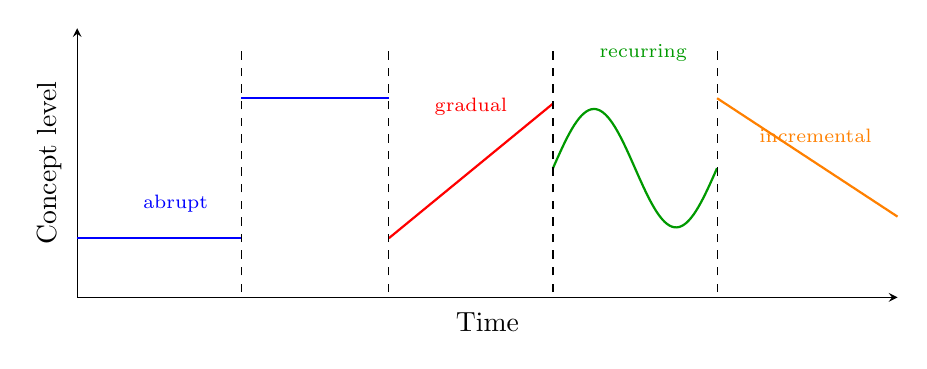
\begin{tikzpicture}
\begin{axis}[
width=12cm,height=5cm,
xlabel={Time}, ylabel={Concept level},
xtick=\empty, ytick=\empty,
xmin=0,xmax=10,ymin=-0.1,ymax=2.4,
axis lines=left, clip=false, grid=major]
\addplot[thick, blue, domain=0:2] {0.45};
\addplot[thick, blue, domain=2:3.8] {1.75};
\node[above, blue] at (axis cs:1.2,0.6) {\scriptsize abrupt};
\addplot[thick, red, domain=3.8:5.8, samples=50] {0.45+1.25*(x-3.8)/2};
\node[above, red] at (axis cs:4.8,1.5) {\scriptsize gradual};
\addplot[thick, green!60!black, domain=5.8:7.8, samples=70] {1.1+0.55*sin(deg(3.14159*(x-5.8)))};
\node[above, green!60!black] at (axis cs:6.9,2.0) {\scriptsize recurring};
\addplot[thick, orange, domain=7.8:10, samples=50] {1.75-1.1*(x-7.8)/2.2};
\node[above, orange] at (axis cs:9.0,1.25) {\scriptsize incremental};
\draw[dashed] (axis cs:2,-0.05)--(axis cs:2,2.25);
\draw[dashed] (axis cs:3.8,-0.05)--(axis cs:3.8,2.25);
\draw[dashed] (axis cs:5.8,-0.05)--(axis cs:5.8,2.25);
\draw[dashed] (axis cs:7.8,-0.05)--(axis cs:7.8,2.25);
\end{axis}
\end{tikzpicture}
\caption{Typical drift regimes in data streams. A useful adaptive ensemble should respond to abrupt drift without becoming unstable under gradual or noisy changes, and should reuse experts under recurring concepts.}
\label{fig:concept_drift_types}
\end{figure}

Several drift detection methods use sliding windows. The main idea is to compare statistics or classifier errors in recent and older windows. VFDT and CVFDT use Hoeffding bounds to build and update decision trees under evolving streams. DDM, EDDM, and EWMA-based detectors monitor the sequence of classification errors. Instance-based and micro-cluster methods represent recent regions of the feature space and discard outdated regions. These methods are effective, but the adaptation rule is often separated from the uncertainty of expert assignment.

\subsection{Ensemble Methods and Dynamic Weighting}
Ensemble learning is a natural solution for drift because different experts can specialize in different regimes. DWM maintains a weighted pool of experts. Each expert has a weight $w_i$, which is reduced by a multiplicative factor $\beta$ when the expert predicts incorrectly. Experts with weights below a threshold $\theta$ can be removed, and new experts can be added when the global ensemble makes mistakes. This strategy is attractive because it is simple and can use many base learners. However, DWM is controlled by several hand-tuned policies: the weight reduction factor, expert creation period, deletion threshold, and the type of expert to be added. Moreover, weights are global and error-driven rather than posterior task responsibilities.

EM-MTE keeps the useful idea of a shared expert library but replaces purely heuristic weighting with a likelihood-based responsibility model. The same component may receive high responsibility for one task and low responsibility for another. This is important in streams where a drift affects one subproblem while another subproblem remains stable.

\subsection{Multi-Task Learning and Mixture of Experts}
Multi-task learning improves generalization by sharing information across related tasks. Mixture-of-experts models combine multiple components through gating or mixing functions. EM is a classical method for estimating mixtures with latent assignments. In the proposed setting, tasks correspond to stream blocks, contexts, or drift-sensitive views, and the latent variable identifies which online component is responsible for explaining a given task sample. Unlike ordinary offline mixtures, the components are incremental learners and the mixture weights are refreshed block by block.

\subsection{Distributional Drift and Stochastic Tracking}
Recent stochastic optimization studies under distributional drift emphasize that the target objective itself may evolve over time. In such problems, the learner must track a moving optimizer. The tracking error can be decomposed into optimization error, stochastic gradient noise, and drift-induced error. This viewpoint is highly relevant to concept drift: if the step size is too small, the learner cannot follow a fast-moving concept; if it is too large, noise dominates. EM-MTE uses responsibility-weighted updates and drift-sensitive mixture changes to balance tracking and stability.

% ---------------------------------------------------------------
\section{Online Components for Concept Drift}
\label{sec:background}
% ================================================================
This section summarizes the online learners used as shared components in
EM-MTE. The goal is not to choose one universal learner, but to build a
heterogeneous component library whose members have different adaptation
behaviors; Section~\ref{sec:proposed} then shows how EM turns this library
into a set of task-specific mixtures rather than a single hand-tuned
ensemble.

\subsection{Data Stream Notation}
Let the incoming stream be
\begin{equation}
D = \{(I_t,L_t)\mid t=1,2,\ldots\},
\end{equation}
where $I_t\in\R^d$ is the feature vector and $L_t\in\{-1,+1\}$ for binary
classification, or $L_t\in\{1,\ldots,C\}$ for multi-class classification.
The stream is split into sequential blocks
\begin{equation}
S = \{s_1,s_2,\ldots,s_B\}.
\end{equation}
Each block can be processed once, and the learner is not allowed to store the
full historical stream.

\begin{definition}[Expandable Stream Schema]
A data stream schema at time $t$ is a feature vector
$I_t=\langle f_1,\ldots,f_d\rangle$. If a new feature $f_{d+1}$ becomes
available, the model can extend the vector as
$\langle f_1,\ldots,f_d,0\rangle$ for older samples and update only the
affected component parameters. This allows the stream representation to
evolve without full retraining.
\end{definition}

\subsection{Linear-Order Online Learners}
Linear-order online learners maintain a weight vector $w_t$ and update it
after each sample. The Perceptron updates on mistakes, Online Gradient
Descent updates according to a differentiable loss, and Passive-Aggressive
(PA) algorithms update strongly when the margin is violated.

For a PA component, the update is derived from
\begin{equation}
 w_{t+1}=\argmin_{w\in\R^d}\frac{1}{2}\|w-w_t\|^2
 \quad \text{s.t.}\quad L_t(w^\top I_t)\geq 1.
 \label{eq:pa_problem}
\end{equation}
Let
\begin{equation}
\ell_t=\max(0,1-L_t w_t^\top I_t).
\end{equation}
The basic PA update is
\begin{equation}
 w_{t+1}=w_t+\frac{\ell_t}{\|I_t\|^2}L_t I_t.
 \label{eq:pa_update_basic}
\end{equation}
PA-I and PA-II introduce an aggressiveness parameter $C$ to control the
maximum correction.

\begin{table}[H]
\centering
\caption{Linear-order online learning components and their drift behavior.}
\label{tab:linear_order}
\renewcommand{\arraystretch}{1.35}
\resizebox{\textwidth}{!}{%
\begin{tabular}{llll}
\toprule
\textbf{Component} & \textbf{Loss} & \textbf{Representative update} & \textbf{Useful drift regime}\\
\midrule
Perceptron~\cite{Irie1988} & $\mathbb{I}[L_t w_t^\top I_t\leq0]$ & $w_{t+1}=w_t+L_t I_t$ on mistakes & abrupt/simple drift\\
OGD~\cite{Zinkevich2003} & $\log(1+e^{-L_t w_t^\top I_t})$ & $w_{t+1}=w_t-\eta_t\nabla\ell_t(w_t)$ & smooth/incremental drift\\
PA~\cite{Crammer2006} & $\max(0,1-L_t w_t^\top I_t)$ & $w_{t+1}=w_t+\frac{\ell_t}{\|I_t\|^2}L_tI_t$ & margin-sensitive drift\\
PA-I~\cite{Crammer2006} & hinge & $\tau_t=\min(C,\ell_t/\|I_t\|^2)$ & noisy gradual drift\\
PA-II~\cite{Crammer2006} & hinge & $\tau_t=\ell_t/(\|I_t\|^2+1/(2C))$ & noisy gradual drift\\
ROMMA~\cite{Li2000} & margin loss & normalized maximum-margin correction & abrupt/recurring drift\\
ALMA~\cite{Gentile2001} & approximate margin loss & normalized $\ell_p$ correction & stable recurring drift\\
\bottomrule
\end{tabular}}
\end{table}

\subsection{Gaussian-Order Online Learners}
Gaussian-order online learners maintain a distribution over the classifier
weights, usually $w\sim\mathcal{N}(\mu,\Sigma)$. The mean vector controls the
classifier, while the covariance matrix represents confidence. A feature
with high uncertainty can be updated more aggressively than a feature with
high confidence.

Confidence-Weighted (CW) learning updates the distribution by minimizing its
KL divergence from the previous distribution subject to a probabilistic
margin constraint:
\begin{equation}
(\mu_{t+1},\Sigma_{t+1})=
\argmin_{\mu,\Sigma}\KL\!\left(\mathcal{N}(\mu,\Sigma)\,\|\,\mathcal{N}(\mu_t,\Sigma_t)\right)
\quad\text{s.t.}\quad
\Prob_{w\sim\mathcal{N}(\mu,\Sigma)}[L_t w^\top I_t\geq0]\geq\phi.
\label{eq:cw_problem}
\end{equation}
A common update form is
\begin{align}
\mu_{t+1} &= \mu_t+\alpha_t L_t\Sigma_t I_t,\label{eq:cw_mu}\\
\Sigma_{t+1} &= \Sigma_t-\beta_t\Sigma_t I_t I_t^\top\Sigma_t,\label{eq:cw_sigma}
\end{align}
where $\alpha_t$ and $\beta_t$ depend on the margin, confidence, and chosen
variant.

\begin{table}[H]
\centering
\caption{Gaussian-order online learning components.}
\label{tab:gaussian_order}
\renewcommand{\arraystretch}{1.35}
\resizebox{\textwidth}{!}{%
\begin{tabular}{llll}
\toprule
\textbf{Component} & \textbf{State} & \textbf{Main idea} & \textbf{Useful drift regime}\\
\midrule
CW~\cite{Dredze2008} & $(\mu,\Sigma)$ & KL-minimal update with confidence margin & low-noise stable drift\\
SCW-I/II~\cite{Wang2012} & $(\mu,\Sigma)$ & soft margin confidence-weighted update & noisy gradual drift\\
AROW~\cite{Crammer2009} & $(\mu,\Sigma)$ & adaptive regularization of weights & robust noisy drift\\
NAROW~\cite{Orabona2012} & $(\mu,\Sigma)$ & normalized adaptive regularization & stable drift with scaling\\
SOP~\cite{CesaBianchi2005} & second-order matrix & second-order Perceptron correction & high-dimensional drift\\
NHERD~\cite{Crammer2010} & distributional state & Gaussian herding with normalization & recurring concepts\\
\bottomrule
\end{tabular}}
\end{table}

The proposed method can use any subset of these components. A heterogeneous
library is useful because concept drift is not a single phenomenon: abrupt
attacks, slow seasonal changes, and recurring concepts may require different
adaptation dynamics. \textbf{This is exactly the gap EM-MTE closes}: instead
of hand-picking one component or a fixed voting weight, Section
\ref{sec:proposed} lets a per-task mixture $\boldsymbol{\pi}^{(r)}$ decide, block by
block, how much each component in Tables~\ref{tab:linear_order} and
\ref{tab:gaussian_order} should be trusted.

% ================================================================
\section{The Proposed EM-MTE Framework}
\label{sec:proposed}
% ================================================================
\subsection{Overview}
The proposed EM-MTE framework treats concept drift adaptation as a
multi-task mixture estimation problem. Each task has its own mixture over a
shared component library. The task-specific mixture is updated by EM, and
the shared components are updated by responsibility-weighted online
learning.

\begin{figure}[H]
\centering
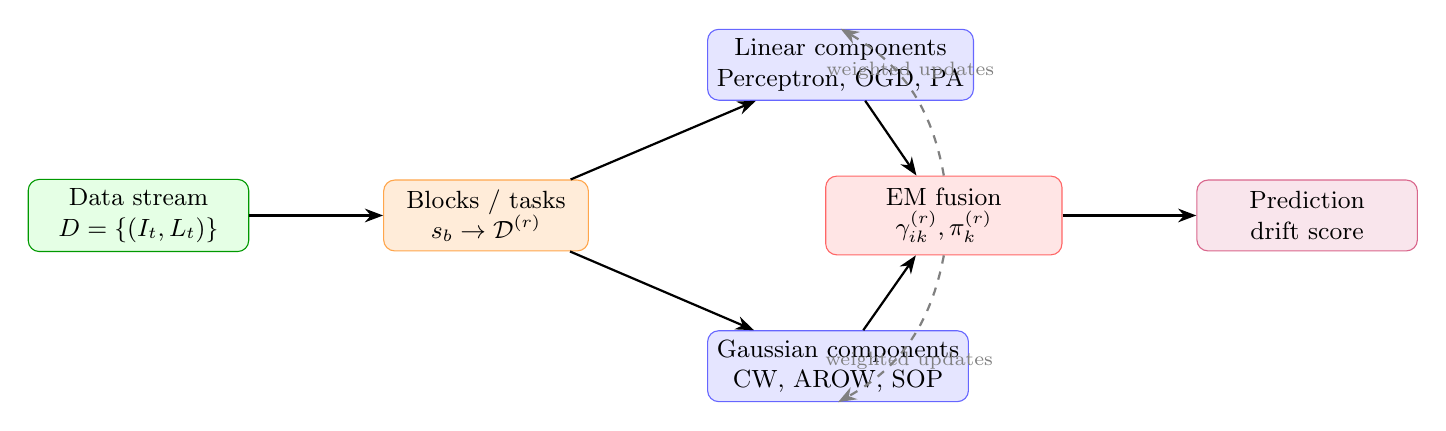
\begin{tikzpicture}[node distance=1.5cm and 1.7cm]
\node[datanode] (stream) {Data stream\\$D=\{(I_t,L_t)\}$};
\node[tasknode, right=of stream] (blocks) {Blocks / tasks\\$s_b\rightarrow\mathcal{D}^{(r)}$};
\node[component, above right=1.0cm and 1.5cm of blocks] (c1) {Linear components\\Perceptron, OGD, PA};
\node[component, below right=1.0cm and 1.5cm of blocks] (c2) {Gaussian components\\CW, AROW, SOP};
\node[emnode, right=3.0cm of blocks] (em) {EM fusion\\$\gamma_{ik}^{(r)},\pi_k^{(r)}$};
\node[outnode, right=of em] (out) {Prediction\\drift score};
\draw[arrow] (stream) -- (blocks);
\draw[arrow] (blocks) -- (c1);
\draw[arrow] (blocks) -- (c2);
\draw[arrow] (c1) -- (em);
\draw[arrow] (c2) -- (em);
\draw[arrow] (em) -- (out);
\draw[dasharrow] (em.south) to[bend left=25] node[below]{\scriptsize weighted updates} (c2.south);
\draw[dasharrow] (em.north) to[bend right=25] node[above]{\scriptsize weighted updates} (c1.north);
\end{tikzpicture}
\caption{Overall architecture of EM-MTE. Stream blocks are interpreted as
tasks or task samples. A shared library of online components produces
predictions, and EM estimates task-specific responsibilities and mixture
weights.}
\label{fig:em_mte_overview}
\end{figure}

\subsection{Task Construction}
Let $\mathcal{T}=\{1,\ldots,T\}$ be the set of tasks. A task may represent a
block, a class-specific view, a feature group, a temporal region, or a
drift-sensitive objective. The dataset assigned to task $r$ is
\begin{equation}
\calD^{(r)}=\{(x_i^{(r)},y_i^{(r)})\}_{i=1}^{N_r}.
\end{equation}
In the simplest implementation, each incoming block $s_b$ is treated as a
temporary task. More structured implementations can define tasks by
application contexts, such as attack type, web page feature group, or sensor
region.

Let the shared component library be
\begin{equation}
\calC=\{C_1,\ldots,C_K\},
\end{equation}
where component $C_k$ has parameters $\theta_k$ and prediction score
$f_k(x;\theta_k)$. The aim is to learn task-specific mixing vectors
\begin{equation}
\boldsymbol{\pi}^{(r)}=(\pi_1^{(r)},\ldots,\pi_K^{(r)}),
\qquad
\pi_k^{(r)}\geq0,
\qquad
\sum_{k=1}^{K}\pi_k^{(r)}=1.
\end{equation}

\subsection{Task-Conditioned Mixture Model}
For task $r$, the predictive distribution is modeled as
\begin{equation}
 p(y_i^{(r)}\mid x_i^{(r)},r)
 =\sum_{k=1}^{K}\pi_k^{(r)}
 p_k(y_i^{(r)}\mid x_i^{(r)},\theta_k).
 \label{eq:mixture_model}
\end{equation}
For a binary margin-based component, a convenient likelihood is
\begin{equation}
 p_k(y_i^{(r)}\mid x_i^{(r)},\theta_k)
 =\sigma\!\left(y_i^{(r)}f_k(x_i^{(r)};\theta_k)\right),
 \qquad
 \sigma(a)=\frac{1}{1+e^{-a}}.
 \label{eq:margin_likelihood}
\end{equation}
Alternatively, any nonnegative loss $\ell_k$ can define a Gibbs likelihood
\begin{equation}
 p_k(y_i^{(r)}\mid x_i^{(r)},\theta_k)
 \propto
 \exp\!\left[-\frac{1}{\tau}\ell_k(\theta_k;(x_i^{(r)},y_i^{(r)}))\right],
 \label{eq:gibbs_likelihood}
\end{equation}
where $\tau>0$ is a temperature parameter. Smaller $\tau$ makes the
responsibility assignment sharper; larger $\tau$ produces smoother sharing
among experts.

\subsection{Latent Responsibility Variables}
Introduce a latent variable $z_i^{(r)}\in\{1,\ldots,K\}$ indicating which
component is responsible for sample $i$ of task $r$. Equivalently, define
binary indicators $z_{ik}^{(r)}=\mathbb{I}[z_i^{(r)}=k]$. The complete-data
likelihood is
\begin{equation}
\calL_c(\Theta)=
\prod_{r=1}^{T}\prod_{i=1}^{N_r}\prod_{k=1}^{K}
\left[
\pi_k^{(r)}p_k(y_i^{(r)}\mid x_i^{(r)},\theta_k)
\right]^{z_{ik}^{(r)}}.
\label{eq:complete_likelihood}
\end{equation}
The complete-data log-likelihood is
\begin{equation}
\log\calL_c(\Theta)=
\sum_{r=1}^{T}\sum_{i=1}^{N_r}\sum_{k=1}^{K}
z_{ik}^{(r)}
\left[
\log\pi_k^{(r)}+
\log p_k(y_i^{(r)}\mid x_i^{(r)},\theta_k)
\right].
\label{eq:complete_log_likelihood}
\end{equation}
The posterior expectation of $z_{ik}^{(r)}$ is the responsibility
\begin{equation}
\gamma_{ik}^{(r)} = \E[z_{ik}^{(r)}\mid x_i^{(r)},y_i^{(r)},\Theta].
\end{equation}

\begin{definition}[Task-Component Responsibility Matrix]
For task $r$ and block $s_b$, the matrix
\begin{equation}
\Gamma^{(r,b)}=\left[\gamma_{ik}^{(r,b)}\right]_{N_r\times K}
\end{equation}
stores the posterior contribution of component $C_k$ to sample $i$. This
matrix is the EM-based replacement for a purely error-correlation or
multiplicative expert matrix.
\end{definition}

\subsection{E-Step}
Given current parameters $\Theta^{(q)}=\{\theta_k^{(q)},\pi_k^{(r,q)}\}$, the
E-step computes
\begin{equation}
\gamma_{ik}^{(r,q)}=
\frac{
\pi_k^{(r,q)}p_k(y_i^{(r)}\mid x_i^{(r)},\theta_k^{(q)})
}{
\sum_{j=1}^{K}\pi_j^{(r,q)}p_j(y_i^{(r)}\mid x_i^{(r)},\theta_j^{(q)})
}.
\label{eq:e_step}
\end{equation}
Using the loss-based likelihood in Eq.~\eqref{eq:gibbs_likelihood}, this
becomes
\begin{equation}
\gamma_{ik}^{(r,q)}=
\frac{
\pi_k^{(r,q)}\exp[-\ell_k(\theta_k^{(q)};(x_i^{(r)},y_i^{(r)}))/\tau]
}{
\sum_{j=1}^{K}\pi_j^{(r,q)}\exp[-\ell_j(\theta_j^{(q)};(x_i^{(r)},y_i^{(r)}))/\tau]
}.
\label{eq:e_step_loss}
\end{equation}
This equation is the main difference from a conventional ensemble. A fixed
ensemble assigns one global weight to each expert, while EM-MTE assigns
task- and sample-dependent responsibilities.

\subsection{M-Step}
The expected complete-data log-likelihood is
\begin{equation}
Q(\Theta\mid\Theta^{(q)})=
\sum_{r=1}^{T}\sum_{i=1}^{N_r}\sum_{k=1}^{K}
\gamma_{ik}^{(r,q)}
\left[
\log\pi_k^{(r)}+
\log p_k(y_i^{(r)}\mid x_i^{(r)},\theta_k)
\right].
\label{eq:q_function}
\end{equation}
For fixed component parameters, maximizing $Q$ with respect to
$\boldsymbol{\pi}^{(r)}$ under the simplex constraint gives
\begin{equation}
\pi_k^{(r,q+1)}=\frac{1}{N_r}\sum_{i=1}^{N_r}\gamma_{ik}^{(r,q)}.
\label{eq:pi_update}
\end{equation}
For better stability in small blocks, a smoothed update can be used:
\begin{equation}
\pi_k^{(r,q+1)}=
\frac{\alpha_0+\sum_{i=1}^{N_r}\gamma_{ik}^{(r,q)}}{K\alpha_0+N_r},
\qquad \alpha_0>0.
\label{eq:pi_smooth_update}
\end{equation}
The shared component parameters are updated by solving
\begin{equation}
\theta_k^{(q+1)}=
\argmin_{\theta_k}
\sum_{r=1}^{T}\sum_{i=1}^{N_r}
\gamma_{ik}^{(r,q)}\ell_k(\theta_k;(x_i^{(r)},y_i^{(r)}))
+\Omega_k(\theta_k),
\label{eq:theta_update_loss}
\end{equation}
where $\Omega_k$ is the regularizer of component $C_k$. For online
components, Eq.~\eqref{eq:theta_update_loss} is implemented as a
responsibility-weighted update.

For example, a responsibility-weighted PA update is
\begin{equation}
 w_{t+1}^{(k)}=w_t^{(k)}+
 \gamma_{tk}^{(r)}\frac{\ell_t^{(k)}}{\|I_t\|^2}L_tI_t.
 \label{eq:weighted_pa_update}
\end{equation}
A responsibility-weighted OGD update is
\begin{equation}
\theta_{k,t+1}=\theta_{k,t}-\eta_t\gamma_{tk}^{(r)}
\nabla_{\theta_k}\ell_k(\theta_{k,t};(I_t,L_t)).
\label{eq:weighted_ogd_update}
\end{equation}
For Gaussian-order components, the responsibility can multiply the update
intensity, e.g.,
\begin{align}
\mu_{t+1}^{(k)} &= \mu_t^{(k)}+
\gamma_{tk}^{(r)}\alpha_t^{(k)} L_t\Sigma_t^{(k)} I_t,\label{eq:weighted_cw_mu}\\
\Sigma_{t+1}^{(k)} &= \Sigma_t^{(k)}-
\gamma_{tk}^{(r)}\beta_t^{(k)}
\Sigma_t^{(k)}I_tI_t^\top\Sigma_t^{(k)}.
\label{eq:weighted_cw_sigma}
\end{align}

\subsection{Prediction}
After the EM update, the score of task $r$ for a new instance $x$ is
\begin{equation}
F^{(r)}(x)=\sum_{k=1}^{K}\pi_k^{(r)}f_k(x;\theta_k).
\label{eq:ensemble_score}
\end{equation}
For binary classification,
\begin{equation}
\hat{y}^{(r)}=\operatorname{sign}(F^{(r)}(x)).
\label{eq:binary_prediction}
\end{equation}
For multi-class classification, component scores can be combined class-wise
and normalized with a softmax.

% ----------------------------------------------------------------
% NOTE ON REORDERING: the drift-detection subsection now comes
% BEFORE the tracking-theoretic subsection, because the tracking
% analysis explicitly refers to the decision rule, the CUSUM
% statistic and the calibrated threshold defined here. In the
% original draft the order was reversed, which produced forward
% references to undefined equations -- exactly the "discontinuity"
% that motivated this revision.
% ----------------------------------------------------------------

\subsection{Responsibility-Based Drift Detection}
\label{sec:drift_detection}
A useful by-product of EM-MTE is that mixture changes can act as drift
indicators. Let $\bm{\pi}_{b}^{(r)}$ be the mixture vector for task $r$ in
block $b$, obtained from Eq.~\eqref{eq:pi_update} (or
Eq.~\eqref{eq:pi_smooth_update}) after $Q$ EM iterations. Define the
mixture-shift score
\begin{equation}
	D_{\pi}^{(r)}(b)=\left\|\bm{\pi}_{b}^{(r)}-\bm{\pi}_{b-1}^{(r)}\right\|_1.
	\label{eq:l1_drift_score}
\end{equation}
Alternatively, a symmetric distributional score can be used:
\begin{equation}
	D_{\JS}^{(r)}(b)=\JS\!\left(\bm{\pi}_{b}^{(r)},\bm{\pi}_{b-1}^{(r)}\right).
	\label{eq:js_drift_score}
\end{equation}

\paragraph{Baseline heuristic (previously undefined).} A first, purely
empirical way to turn $D_\pi^{(r)}(b)$ into an alarm is to track its running
mean $\bar D_\pi^{(r)}$ and running standard deviation $s_D^{(r)}$ over the
past $W$ blocks and raise an alarm whenever the current value exceeds a
fixed number $\kappa>0$ of standard deviations above the mean:
\begin{equation}
	\text{drift}^{(r)}_{\text{heur}}(b) =
	\mathbb{I}\!\left[D_\pi^{(r)}(b) \;\geq\; \bar D_\pi^{(r)} + \kappa\, s_D^{(r)}\right].
	\label{eq:drift_threshold}
\end{equation}
Eq.~\eqref{eq:drift_threshold} is simple to implement but gives no
finite-sample control over the false-alarm probability: $\kappa$ is a free
knob tuned by hand, and its relation to $K$ (the number of components) and
$N_r^{(b)}$ (the block size) is left implicit. The rest of this subsection
replaces Eq.~\eqref{eq:drift_threshold} with a calibrated rule that has an
explicit, provable false-alarm guarantee, and shows that
Eq.~\eqref{eq:drift_threshold} is recovered as its large-sample special
case.

Rather than relying only on an empirically tracked mean and standard
deviation, we now derive a finite-sample threshold with a guaranteed
false-alarm level, and quantify the resulting detection power.

\begin{assumption}[Bounded, conditionally independent responsibilities within a block]
	\label{as:bounded_indep_v2}
	Within block $s_b$, the responsibility vectors
	$\{\gamma_{i,\cdot}^{(r,b)}\}_{i=1}^{N_r^{(b)}}$ that produce
	$\bm\pi_b^{(r)}$ via Eq.~\eqref{eq:pi_update} are conditionally
	independent given $\Theta^{(q)}$, with each coordinate
	$\gamma_{ik}^{(r,b)}\in[0,1]$, where $N_r^{(b)}$ is the number of samples
	of task $r$ in block $b$.
\end{assumption}

\begin{lemma}[Concentration of the block mixture estimate]
	\label{lem:hoeffding_v2}
	Under Assumption~\ref{as:bounded_indep_v2}, let
	$\bm\pi_b^{(r),\star}=\E[\bm\pi_b^{(r)}]$ denote the population-level
	mixture for block $b$. Then, for every $\varepsilon>0$,
	\begin{equation}
		\mathbb{P}\!\left(\left\|\bm\pi_b^{(r)}-\bm\pi_b^{(r),\star}\right\|_\infty\geq\varepsilon\right)
		\leq 2K\exp\!\left(-2N_r^{(b)}\varepsilon^2\right),
		\label{eq:conc_infty}
	\end{equation}
	and consequently, using $\|\mathbf v\|_1\leq K\|\mathbf v\|_\infty$,
	\begin{equation}
		\mathbb{P}\!\left(\left\|\bm\pi_b^{(r)}-\bm\pi_b^{(r),\star}\right\|_1\geq K\varepsilon\right)
		\leq 2K\exp\!\left(-2N_r^{(b)}\varepsilon^2\right).
		\label{eq:conc_l1}
	\end{equation}
\end{lemma}
\begin{proof}
	Each coordinate
	$\pi_{b,k}^{(r)}=\frac{1}{N_r^{(b)}}\sum_{i=1}^{N_r^{(b)}}\gamma_{ik}^{(r,b)}$
	is an average of $N_r^{(b)}$ conditionally independent terms bounded in
	$[0,1]$; Hoeffding's inequality gives
	$\mathbb{P}(|\pi_{b,k}^{(r)}-\pi_{b,k}^{(r),\star}|\geq\varepsilon)\leq2\exp(-2N_r^{(b)}\varepsilon^2)$,
	and a union bound over $k=1,\ldots,K$ yields Eq.~\eqref{eq:conc_infty}.
	Eq.~\eqref{eq:conc_l1} follows from the $\ell_1$--$\ell_\infty$ norm
	inequality on $\mathbb{R}^K$.
\end{proof}

\begin{proposition}[Calibrated threshold with controlled false-alarm rate]
	\label{prop:fa_v2}
	Assume no drift occurs between blocks $b-1$ and $b$ for task $r$, so
	$\bm\pi_{b-1}^{(r),\star}=\bm\pi_{b}^{(r),\star}=\bm\pi^\star$. Let
	$N_{\min}=\min\{N_r^{(b-1)},N_r^{(b)}\}$ and fix a target false-alarm
	level $\alpha\in(0,1)$. Set
	\begin{equation}
		\tau_\alpha(b) = K\sqrt{\frac{2\ln(4K/\alpha)}{N_{\min}}}.
		\label{eq:tau_alpha_v2}
	\end{equation}
	Then
	\begin{equation}
		\mathbb{P}\!\left(D_\pi^{(r)}(b)\geq\tau_\alpha(b)\right)\leq\alpha.
		\label{eq:fa_bound_v2}
	\end{equation}
\end{proposition}
\begin{proof}
	By the triangle inequality,
	$D_\pi^{(r)}(b)\leq\|\bm\pi_b^{(r)}-\bm\pi^\star\|_1+\|\bm\pi_{b-1}^{(r)}-\bm\pi^\star\|_1$.
	Applying Eq.~\eqref{eq:conc_l1} to both terms with
	$\varepsilon=\tau_\alpha(b)/(2K)$ and $N_{\min}$ samples, and taking a
	union bound over the two events, gives
	$\mathbb{P}(D_\pi^{(r)}(b)\geq\tau_\alpha(b))\leq4K\exp\!\left(-N_{\min}\tau_\alpha(b)^2/(2K^2)\right)=\alpha$
	after substituting Eq.~\eqref{eq:tau_alpha_v2}.
\end{proof}

\begin{proposition}[Detection power]
	\label{prop:power_v2}
	Suppose a true drift occurs at block $b^\star$ with
	$\|\bm\pi_{b^\star}^{(r),\star}-\bm\pi_{b^\star-1}^{(r),\star}\|_1=\delta>2\tau_\alpha(b^\star)$.
	Then, using the same threshold $\tau_\alpha(b^\star)$ from
	Eq.~\eqref{eq:tau_alpha_v2},
	\begin{equation}
		\mathbb{P}\!\left(D_\pi^{(r)}(b^\star)\geq\tau_\alpha(b^\star)\right)\geq1-\alpha.
		\label{eq:power_bound_v2}
	\end{equation}
\end{proposition}
\begin{proof}
	By the reverse triangle inequality,
	$D_\pi^{(r)}(b^\star)\geq\delta-\left(\|\bm\pi_{b^\star}^{(r)}-\bm\pi_{b^\star}^{(r),\star}\|_1+\|\bm\pi_{b^\star-1}^{(r)}-\bm\pi_{b^\star-1}^{(r),\star}\|_1\right)$.
	By Eq.~\eqref{eq:conc_l1} and a union bound (as in
	Proposition~\ref{prop:fa_v2}), the bracketed sum is below
	$\tau_\alpha(b^\star)$ with probability at least $1-\alpha$; on this
	event $D_\pi^{(r)}(b^\star)>\delta-\tau_\alpha(b^\star)>\tau_\alpha(b^\star)$
	since $\delta>2\tau_\alpha(b^\star)$.
\end{proof}

Propositions~\ref{prop:fa_v2}--\ref{prop:power_v2} give a fully calibrated
replacement for the running mean/standard-deviation rule in
Eq.~\eqref{eq:drift_threshold}: the false-alarm probability is controlled at
level $\alpha$ irrespective of $K$ or $N_{\min}$, and any drift with
$\delta>2\tau_\alpha(b)=2K\sqrt{2\ln(4K/\alpha)/N_{\min}}$ is detected with
probability at least $1-\alpha$. The minimum detectable drift shrinks as
$\mathcal{O}(K/\sqrt{N_{\min}})$, making the earlier heuristic
$\bar D_\pi^{(r)}+\kappa s_D^{(r)}$ (Eq.~\eqref{eq:drift_threshold}) a special
case that can be recovered asymptotically (for large numbers of past
blocks, the running mean and standard deviation converge to $0$ and a value
proportional to $\tau_\alpha(b)$, respectively, by
Lemma~\ref{lem:hoeffding_v2}), but without an explicit, finite-sample
$\alpha$-guarantee.

\paragraph{Extension to the Jensen--Shannon score.} Since $D_{\JS}^{(r)}(b)$
and $D_\pi^{(r)}(b)$ measure the same underlying shift, they can be related
through the classical inequality of Lin~\cite{Lin1991},
\begin{equation}
	D_{\JS}^{(r)}(b)\;\leq\;\tfrac{1}{2}\ln 2\cdot D_\pi^{(r)}(b),
	\label{eq:js_l1_link}
\end{equation}
so that $D_\pi^{(r)}(b)<\tau_\alpha(b)$ implies
$D_{\JS}^{(r)}(b)<\tfrac{1}{2}\ln2\cdot\tau_\alpha(b)$. Hence, the calibrated
threshold $\tau_\alpha(b)$ derived for the $\ell_1$ score in
Eq.~\eqref{eq:tau_alpha_v2} directly yields a valid (conservative) threshold
$\tau_\alpha^{\JS}(b)=\tfrac{1}{2}\ln2\cdot\tau_\alpha(b)$ for $D_{\JS}^{(r)}(b)$
with the same false-alarm guarantee of Proposition~\ref{prop:fa_v2}.

\paragraph{Cumulative statistic for gradual and recurring drift.}
Single-block comparisons are well suited to abrupt drift but may miss slow,
incremental drift whose per-block increment stays below $\tau_\alpha(b)$. We
therefore track, in parallel, a CUSUM-style cumulative statistic~\cite{Page1954}
\begin{equation}
	G^{(r,b)}=\max\!\left(0,\;G^{(r,b-1)}+D_\pi^{(r)}(b)-\nu\right),\qquad G^{(r,0)}=0,
	\label{eq:cusum_v2}
\end{equation}
with slack $\nu\in(0,\tau_\alpha(b))$. Standard CUSUM theory guarantees that,
for a sustained per-block drift rate $\bar\delta>\nu$, the expected number of
blocks to detection is $\mathcal{O}(h/(\bar\delta-\nu))$ for control limit
$h$, while the in-control average run length grows exponentially in $h$,
complementing Proposition~\ref{prop:power_v2} for the recurring/incremental
drift regimes.

\paragraph{Decision rule.} The heuristic alarm in
Eq.~\eqref{eq:drift_threshold} is replaced by the calibrated rule
\begin{equation}
	\text{drift}^{(r)}(b) \;=\;
	\mathbb{I}\!\left[D_\pi^{(r)}(b)\geq\tau_\alpha(b)\right]
	\;\vee\;
	\mathbb{I}\!\left[G^{(r,b)}\geq h\right],
	\label{eq:decision_rule_v2}
\end{equation}
which controls the block-level false-alarm probability at $\alpha$
(Proposition~\ref{prop:fa_v2}) for abrupt shifts, while retaining
sensitivity to gradual drift through $G^{(r,b)}$, and can equivalently be
evaluated on $D_{\JS}^{(r)}(b)$ via the threshold $\tau_\alpha^{\JS}(b)$ from
Eq.~\eqref{eq:js_l1_link}.

% ----------------------------------------------------------------
\subsection{Tracking-Theoretic Analysis: Lag Error and Misadjustment}
\label{sec:tracking_theory}

The detection rule of Section~\ref{sec:drift_detection}
(Eq.~\eqref{eq:decision_rule_v2}) answers \emph{when} drift has occurred. We
now give a complementary, adaptive-filtering-style theory of \emph{how well}
the mixture estimator $\pi_k^{(r)}$ can track a continuously drifting
concept, in the spirit of the classical misadjustment-versus-lag trade-off in
LMS/RLS tracking analysis~\cite{WidrowStearns1985,Sayed2003,Haykin2002}. This
yields a closed-form optimal adaptation rate and identifies the exact regime
in which the plain block estimator of Eq.~\eqref{eq:pi_update} is itself
already optimal.

\subsubsection{A Random-Walk Model of Concept Drift}

Fix a task $r$ and component $k$, and drop the $(r,k)$ superscripts where
unambiguous. Let $\pi^\star(b)$ denote the (unobservable) \emph{true}
population mixing weight at block $b$. Following the standard
nonstationary-environment model used in adaptive filter tracking
theory~\cite{WidrowStearns1985}, we model gradual concept drift as a random
walk:
\begin{equation}
\pi^\star(b) = \pi^\star(b-1) + \eta(b), \qquad \mathbb{E}[\eta(b)]=0,\ \; \operatorname{Var}[\eta(b)]=\sigma_\eta^2,
	\label{eq:rw_model}
\end{equation}
with $\{\eta(b)\}$ i.i.d.\ and independent of all sampling noise. Here
$\sigma_\eta^2$ is the \emph{drift rate}: it quantifies how fast the concept
moves per block, independently of any estimator.

The block estimator of Eq.~\eqref{eq:pi_update},
$\bar\pi(b)=\frac{1}{N_r^{(b)}}\sum_i\gamma_{ik}^{(r,b)}$, is a noisy
observation of $\pi^\star(b)$:
\begin{equation}
\bar\pi(b) = \pi^\star(b) + v(b), \qquad \mathbb{E}[v(b)]=0,\ \; \operatorname{Var}[v(b)]=\sigma_v^2(b),
	\label{eq:obs_model}
\end{equation}
where, since $\gamma_{ik}^{(r,b)}\in[0,1]$, Popoviciu's inequality on
bounded variables gives the sampling-noise bound
\begin{equation}
	\sigma_v^2(b) \;\leq\; \frac{1}{4N_r^{(b)}}.
	\label{eq:sigma_v_bound}
\end{equation}

\subsubsection{A General Recursive Tracking Estimator}

We generalize the raw block estimator to a first-order recursive
(exponentially weighted) tracker, exactly analogous to an LMS-type adaptive
filter with step size $\mu\in(0,1]$:
\begin{equation}
	\hat\pi(b) = (1-\mu)\,\hat\pi(b-1) + \mu\,\bar\pi(b).
	\label{eq:ewma_tracker}
\end{equation}
Setting $\mu=1$ recovers exactly the plain block estimator
$\hat\pi(b)=\bar\pi(b)$ used in Eq.~\eqref{eq:pi_update}; smaller $\mu$
corresponds to smoothing across blocks (a forgetting-factor / RLS-style
update), trading responsiveness for noise reduction.

\begin{proposition}[Lag--Misadjustment Decomposition]
	\label{prop:tracking_mse}
	Let $e(b)=\hat\pi(b)-\pi^\star(b)$ under the models
	\eqref{eq:rw_model}--\eqref{eq:obs_model}, with $\sigma_v^2(b)\equiv\sigma_v^2$
	constant across blocks (e.g., fixed block size). In steady state, the
	tracking mean-squared error satisfies
	\begin{equation}
		\sigma_e^2 \;=\; \frac{\mu^2\sigma_v^2 + (1-\mu)^2\sigma_\eta^2}{\mu(2-\mu)}
		\;\;\xrightarrow{\ \mu\ \text{small}\ }\;\;
		\underbrace{\frac{\mu}{2}\,\sigma_v^2}_{\text{misadjustment}} \;+\; \underbrace{\frac{\sigma_\eta^2}{2\mu}}_{\text{lag error}}.
		\label{eq:mse_decomp}
	\end{equation}
\end{proposition}
\begin{proof}
	From Eqs.~\eqref{eq:rw_model}--\eqref{eq:ewma_tracker},
	\[
	e(b) = (1-\mu)\hat\pi(b-1)+\mu\bar\pi(b)-\pi^\star(b)
	= (1-\mu)\big[\hat\pi(b-1)-\pi^\star(b-1)\big] - (1-\mu)\eta(b) + \mu v(b)
	= (1-\mu)e(b-1) + \mu v(b) - (1-\mu)\eta(b).
	\]
Since $\eta(b)$ and $v(b)$ are independent of $e(b-1)$ (both are innovations
arriving at block $b$) and independent of each other, taking variances and
imposing steady state ($\operatorname{Var}[e(b)]=\operatorname{Var}[e(b-1)]=\sigma_e^2$)
gives
	\[
	\sigma_e^2 = (1-\mu)^2\sigma_e^2 + \mu^2\sigma_v^2 + (1-\mu)^2\sigma_\eta^2 .
	\]
	Solving for $\sigma_e^2$ and using $1-(1-\mu)^2=\mu(2-\mu)$ yields
	Eq.~\eqref{eq:mse_decomp}. The small-$\mu$ approximation follows from
	$(1-\mu)^2\approx1$ and $2-\mu\approx2$.
\end{proof}

Eq.~\eqref{eq:mse_decomp} is the precise formal statement of the phenomenon
the reviewer intuition points to: a large $\mu$ (fast adaptation, e.g.\
small blocks or an aggressive forgetting factor) tracks the drift with
little \emph{lag} but inflates variance from sampling noise — this excess
error is exactly the \textbf{misadjustment} term, in the same sense as in
LMS adaptive filter theory. A small $\mu$ suppresses misadjustment but the
estimator lags behind a moving concept, inflating the \textbf{lag error}
term. Neither extreme is optimal; effective drift tracking requires
balancing the two, not simply reacting to every fluctuation.

\begin{corollary}[Optimal Adaptation Rate]
	\label{cor:optimal_mu}
	The step size minimizing the (small-$\mu$) tracking MSE in
	Eq.~\eqref{eq:mse_decomp} is
	\begin{equation}
		\mu^\star = \frac{\sigma_\eta}{\sigma_v} \quad \text{(clipped to $[0,1]$)},
		\label{eq:mu_star}
	\end{equation}
	attaining the minimum achievable tracking error
	\begin{equation}
		\sigma_{e,\min}^2 = \sigma_\eta\,\sigma_v .
		\label{eq:mse_min}
	\end{equation}
\end{corollary}
\begin{proof}
	Differentiating the right-hand side of Eq.~\eqref{eq:mse_decomp} with
	respect to $\mu$ and setting it to zero gives
	$\sigma_v^2/2 - \sigma_\eta^2/(2\mu^2)=0$, i.e.\
	$\mu^2=\sigma_\eta^2/\sigma_v^2$, which gives Eq.~\eqref{eq:mu_star} (the
	positive root, and clipped to $1$ if $\sigma_\eta\geq\sigma_v$, since
	$\mu\le1$ by construction). Substituting $\mu^\star$ back into
	Eq.~\eqref{eq:mse_decomp} gives
	$\sigma_{e,\min}^2 = \frac{1}{2}\frac{\sigma_\eta}{\sigma_v}\sigma_v^2 + \frac{\sigma_\eta^2}{2}\frac{\sigma_v}{\sigma_\eta} = \sigma_\eta\sigma_v$.
\end{proof}

\begin{remark}[When is the plain block estimator already optimal?]
	\label{rem:mu_equals_one}
	Combining Eq.~\eqref{eq:mu_star} with the sampling-noise bound
	\eqref{eq:sigma_v_bound}, $\mu^\star\ge1$ — i.e.\ no cross-block
	smoothing is needed and the plain estimator $\hat\pi(b)=\bar\pi(b)$ of
	Eq.~\eqref{eq:pi_update} is itself MSE-optimal — precisely when
	\begin{equation}
		N_r^{(b)} \;\geq\; \frac{1}{4\sigma_\eta^2}.
		\label{eq:n_condition}
	\end{equation}
	Conversely, when blocks are too small relative to the drift rate
	$\sigma_\eta$ (i.e.\ $N_r^{(b)} < 1/(4\sigma_\eta^2)$), Eq.~\eqref{eq:pi_update}
	is sub-optimal and should be replaced by the recursive tracker of
	Eq.~\eqref{eq:ewma_tracker} with $\mu=\mu^\star=\sigma_\eta/\sigma_v$
	estimated online. Lemma~\ref{lem:online_scales} below makes this
	estimation step precise.
\end{remark}

\begin{remark}[Consequence for the detection threshold]
	\label{rem:noise_floor}
	Corollary~\ref{cor:optimal_mu} also supplies a principled \emph{noise
	floor} for the detector of Section~\ref{sec:drift_detection}: since even
	the best possible tracker cannot resolve drift below
	$\sigma_{e,\min}=\sqrt{\sigma_\eta\sigma_v}$, the CUSUM slack $\nu$ in
	Eq.~\eqref{eq:cusum_v2} should satisfy $\nu \gtrsim \sigma_{e,\min}$, and
	the false-alarm threshold $\tau_\alpha(b)$ of Eq.~\eqref{eq:tau_alpha_v2}
	should be interpreted relative to this floor rather than assumed to
	shrink to zero as $N_r^{(b)}\to\infty$: for a genuinely drifting
	environment ($\sigma_\eta>0$), the block size cannot be grown
	indefinitely to suppress false alarms without simultaneously
	reintroducing lag error, by Eq.~\eqref{eq:mse_decomp}.
\end{remark}

\subsubsection{Online Estimation of the Drift and Noise Scales}
\label{sec:online_scales}

Remark~\ref{rem:mu_equals_one} calls for $\sigma_\eta$ and $\sigma_v$
``estimated online''; the following lemma turns this into concrete,
computable estimators and gives them a concentration guarantee, so that the
adaptive step size $\mu^\star=\sigma_\eta/\sigma_v$ is not just a
theoretical quantity but something the algorithm can actually set.

\begin{lemma}[Online Estimation of Drift and Noise Scales]
	\label{lem:online_scales}
	Fix task $r$ and component $k$. At block $b$, define the plug-in
	noise-scale estimator from the within-block spread of the responsibilities,
	\begin{equation}
		\hat\sigma_v^2(b) = \frac{1}{N_r^{(b)}\big(N_r^{(b)}-1\big)}
		\sum_{i=1}^{N_r^{(b)}} \Big(\gamma_{ik}^{(r,b)}-\bar\pi_k(b)\Big)^2,
		\label{eq:sigma_v_hat}
	\end{equation}
	which is the sample variance of the block mean $\bar\pi_k(b)$, and let
	$W\ge2$ be a burn-in window of consecutive blocks. Define the bias-corrected
	drift-scale estimator
	\begin{equation}
		\hat\sigma_\eta^2 = \max\!\left(0,\;
		\frac{1}{W-1}\sum_{b'=b-W+1}^{b-1}
		\big(\bar\pi_k(b'+1)-\bar\pi_k(b')\big)^2
		\;-\;\frac{2}{W}\sum_{b'=b-W+1}^{b}\hat\sigma_v^2(b')
		\right).
		\label{eq:sigma_eta_hat}
	\end{equation}
	Then, under Assumption~\ref{as:bounded_indep_v2} and the random-walk
	model~\eqref{eq:rw_model}--\eqref{eq:obs_model}:
	\begin{enumerate}
		\item[(i)] $\hat\sigma_v^2(b)$ is an unbiased estimator of
		$\sigma_v^2(b)$, and by Hoeffding's inequality on the bounded
		summands $\gamma_{ik}^{(r,b)}\in[0,1]$,
		\begin{equation}
			\Prob\Big(\big|\hat\sigma_v^2(b)-\sigma_v^2(b)\big|\geq\varepsilon\Big)
			\leq 2\exp\!\left(-\frac{N_r^{(b)}\varepsilon^2}{2}\right)\quad\text{for } N_r^{(b)}\text{ large.}
			\label{eq:sigma_v_conc}
		\end{equation}
		\item[(ii)] Since $\bar\pi_k(b'+1)-\bar\pi_k(b')=\eta(b'+1)+v(b'+1)-v(b')$
		and $\eta,v$ are mutually independent, $\E\big[(\bar\pi_k(b'+1)-\bar\pi_k(b'))^2\big]=\sigma_\eta^2+2\sigma_v^2$, so
		$\hat\sigma_\eta^2$ in Eq.~\eqref{eq:sigma_eta_hat} is an asymptotically
		unbiased (as $W\to\infty$) estimator of $\sigma_\eta^2$, and a union
		bound combining $W$ applications of a Hoeffding-type tail bound on
		the bounded increments gives, for any $\varepsilon>0$,
		\begin{equation}
			\Prob\Big(\big|\hat\sigma_\eta^2-\sigma_\eta^2\big|\geq\varepsilon\Big)
			\leq 2(W+1)\exp\!\left(-c\,\varepsilon^2\, N_{\min}\right)
			\label{eq:sigma_eta_conc}
		\end{equation}
		for a universal constant $c>0$ and $N_{\min}=\min_{b'} N_r^{(b')}$
		over the burn-in window.
	\end{enumerate}
\end{lemma}
\begin{proof}
	(i) $\hat\sigma_v^2(b)$ is the usual sample-variance-of-the-mean
	estimator computed from $N_r^{(b)}$ conditionally independent, $[0,1]$-bounded
	terms (Assumption~\ref{as:bounded_indep_v2}); unbiasedness is the
	standard property of the sample variance divided by $N_r^{(b)}(N_r^{(b)}-1)$,
	and the concentration in Eq.~\eqref{eq:sigma_v_conc} follows from a
	Hoeffding-Bernstein bound for U-statistics of bounded variables. (ii)
	The identity for $\E[(\bar\pi_k(b'+1)-\bar\pi_k(b'))^2]$ follows directly
	from Eqs.~\eqref{eq:rw_model}--\eqref{eq:obs_model} and independence of
	$\eta(\cdot)$ and $v(\cdot)$ across blocks. Each increment
	$\bar\pi_k(b'+1)-\bar\pi_k(b')$ is itself an average of bounded,
	conditionally independent responsibilities (via Eq.~\eqref{eq:pi_update})
	minus another such average, hence bounded in $[-1,1]$ and concentrated
	around its mean at rate governed by $N_{\min}$; summing $W$ such terms
	and applying a union bound over the $W$ increments together with the
	$W+1$ variance estimates $\hat\sigma_v^2(b')$ gives
	Eq.~\eqref{eq:sigma_eta_conc}, with $c$ absorbing the constants from the
	individual Hoeffding bounds.
\end{proof}

\begin{corollary}[Unified Design Rule for $\mu$, $\nu$, and $h$]
	\label{cor:unified_design}
	Given the estimates $\hat\sigma_v(b)=\sqrt{\hat\sigma_v^2(b)}$ and
	$\hat\sigma_\eta=\sqrt{\hat\sigma_\eta^2}$ from Lemma~\ref{lem:online_scales},
	set
	\begin{equation}
		\hat\mu^\star = \operatorname{clip}\!\left(\frac{\hat\sigma_\eta}{\hat\sigma_v(b)},\,0,\,1\right),
		\qquad
		\hat\sigma_{e,\min} = \sqrt{\hat\sigma_\eta\,\hat\sigma_v(b)},
		\qquad
		\nu = c_\nu\,\hat\sigma_{e,\min},\ \ c_\nu\in(0,1),
		\label{eq:unified_rule}
	\end{equation}
	and choose the CUSUM control limit $h$ to meet a target average run
	length $\mathrm{ARL}_0$ in the drift-free regime. Then: (a) by
	Corollary~\ref{cor:optimal_mu}, $\hat\mu^\star$ is a consistent estimator
	of the mixture-tracking-optimal step size $\mu^\star$ as
	$N_{\min},W\to\infty$, by Eqs.~\eqref{eq:sigma_v_conc}--\eqref{eq:sigma_eta_conc};
	(b) the resulting slack satisfies $\nu<\tau_\alpha(b)$ whenever
	$c_\nu\hat\sigma_{e,\min}<\tau_\alpha(b)$, which holds for any
	$c_\nu<1$ once the block size satisfies the condition of
	Remark~\ref{rem:noise_floor} together with Eq.~\eqref{eq:tau_alpha_v2},
	so the CUSUM statistic of Eq.~\eqref{eq:cusum_v2} remains
	well-posed; and (c) $\mu$, $\nu$, and $h$ are therefore set from the
	\emph{same} pair of online scale estimates
	$(\hat\sigma_\eta,\hat\sigma_v)$, rather than being tuned as three
	independent free parameters.
\end{corollary}
\begin{proof}
	(a) follows directly from plugging the concentration results of
	Lemma~\ref{lem:online_scales} into the continuous map
	$(\sigma_\eta,\sigma_v)\mapsto\sigma_\eta/\sigma_v$ on a domain bounded
	away from $\sigma_v=0$ (guaranteed for $N_r^{(b)}$ finite by
	Eq.~\eqref{eq:sigma_v_bound}), which is Lipschitz there, so consistency
	of $(\hat\sigma_\eta,\hat\sigma_v)$ transfers to consistency of
	$\hat\mu^\star$. (b) is an immediate rearrangement of the stated
	inequality using the definition of $\nu$ in Eq.~\eqref{eq:unified_rule}.
	(c) is definitional.
\end{proof}

% ----------------------------------------------------------------
\subsection{Diversity Regularization}
The previous correlation-based ensemble idea can be retained as an optional
diversity regularizer. Let $\Sigma_e^{(r)}$ be the error covariance matrix of
components for task $r$. The regularized objective is
\begin{equation}
\mathcal{J}(\Theta)=
-Q(\Theta\mid\Theta^{(q)})+
\rho\sum_{r=1}^{T}(\bm{\pi}^{(r)})^\top\Sigma_e^{(r)}\bm{\pi}^{(r)},
\label{eq:diversity_regularized_objective}
\end{equation}
where $\rho\geq0$. When $\rho=0$, the method is the pure EM-based multi-task
ensemble. When $\rho>0$, the mixture discourages assigning large weights to
highly correlated error-producing components.

\begin{remark}[Choosing $\rho$]
Because $\mathcal J(\Theta)$ trades exact EM optimality against diversity,
$\rho$ should be tied to how noisy the responsibilities already are: when
$\hat\sigma_v(b)$ from Eq.~\eqref{eq:sigma_v_hat} is large (few samples per
block, unreliable responsibilities), a larger $\rho$ regularizes the mixture
toward decorrelated components and partially compensates for the
sampling-noise term in Eq.~\eqref{eq:mse_decomp}; when $\hat\sigma_v(b)$ is
small, $\rho$ can be relaxed toward $0$ so that the mixture is driven mainly
by the EM fit.
\end{remark}

\subsection{Block-Wise Online Procedure}
In streaming mode, EM is performed for a small number of iterations per
block. The responsibility and mixture estimates from block $b-1$ initialize
block $b$, enabling warm-started adaptation. Following
Remark~\ref{rem:mu_equals_one} and Corollary~\ref{cor:unified_design}, the
plain block update of Eq.~\eqref{eq:pi_update} is used whenever
Eq.~\eqref{eq:n_condition} holds, and the EWMA tracker of
Eq.~\eqref{eq:ewma_tracker} with $\mu=\hat\mu^\star$ is used otherwise.

\begin{figure}[H]
\centering
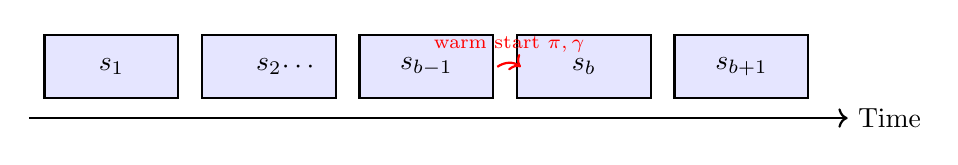
\begin{tikzpicture}[scale=1.0]
\foreach \i/\label in {0/$s_1$,2/$s_2$,4/$s_{b-1}$,6/$s_b$,8/$s_{b+1}$}{
\draw[thick,fill=blue!10] (\i,0) rectangle (\i+1.7,0.8);
\node at (\i+0.85,0.4) {\label};}
\node at (3.25,0.4) {$\cdots$};
\draw[->,thick,red] (5.75,0.4) to[bend left=35] node[above]{\scriptsize warm start $\pi,\gamma$} (6.05,0.4);
\draw[->,thick] (-0.2,-0.25)--(10.2,-0.25) node[right]{Time};
\end{tikzpicture}
\caption{Block-wise EM update. The posterior mixture from the previous block
initializes the current block, reducing adaptation delay.}
\label{fig:blockwise_em}
\end{figure}

\begin{algorithm}[H]
\caption{EM-MTE: EM-Based Multi-Task Ensemble for Data Streams}
\label{alg:em_mte}
\begin{algorithmic}[1]
\REQUIRE Stream blocks $\{s_b\}_{b=1}^{B}$; number of components $K$; task
constructor $\mathcal{A}$; EM iterations $Q$; temperature $\tau$; false-alarm
level $\alpha$; burn-in window $W$.
\ENSURE Predictions $\hat{y}_t$, component parameters
$\{\theta_k\}_{k=1}^{K}$, task mixtures $\{\bm{\pi}^{(r)}\}_{r=1}^{T}$, drift
alarms.
\STATE Initialize components $C_1,\ldots,C_K$ and parameters $\theta_k^{(0)}$.
\STATE Initialize $\pi_k^{(r,0)}\leftarrow1/K$ for all tasks and components; $G^{(r,0)}\leftarrow0$.
\FOR{each incoming block $s_b$}
  \STATE Construct or update tasks $\{\calD_b^{(r)}\}_{r=1}^{T_b}=\mathcal{A}(s_b)$.
  \STATE Warm-start $\bm{\pi}_b^{(r)}$ from the closest previous task mixture if available.
  \FOR{$q=0,1,\ldots,Q-1$}
    \FOR{each task $r$, sample $i$, and component $k$}
      \STATE Compute $p_k(y_i^{(r)}\mid x_i^{(r)},\theta_k^{(q)})$ or the loss $\ell_k$.
      \STATE Compute responsibility $\gamma_{ik}^{(r,q)}$ using Eq.~\eqref{eq:e_step} or Eq.~\eqref{eq:e_step_loss}.
    \ENDFOR
    \FOR{each task $r$ and component $k$}
      \STATE Estimate $\hat\sigma_v^2(b)$, $\hat\sigma_\eta^2$ via Eqs.~\eqref{eq:sigma_v_hat}--\eqref{eq:sigma_eta_hat}.
      \IF{$N_r^{(b)}\geq 1/(4\hat\sigma_\eta^2)$ \textbf{(Eq.~\eqref{eq:n_condition})}}
        \STATE Update $\pi_k^{(r,q+1)}$ using Eq.~\eqref{eq:pi_update} or Eq.~\eqref{eq:pi_smooth_update}.
      \ELSE
        \STATE Compute $\hat\mu^\star$ via Eq.~\eqref{eq:unified_rule} and update $\pi_k^{(r,q+1)}$ using the EWMA tracker of Eq.~\eqref{eq:ewma_tracker}.
      \ENDIF
    \ENDFOR
    \FOR{each component $k$}
      \STATE Update $\theta_k^{(q+1)}$ by the responsibility-weighted online rule in Eq.~\eqref{eq:theta_update_loss}.
    \ENDFOR
  \ENDFOR
  \STATE Predict each new sample using Eq.~\eqref{eq:ensemble_score} and Eq.~\eqref{eq:binary_prediction}.
  \STATE Compute $D_\pi^{(r)}(b)$ via Eq.~\eqref{eq:l1_drift_score} (or $D_{\JS}^{(r)}(b)$ via Eq.~\eqref{eq:js_drift_score}).
  \STATE Set $\tau_\alpha(b)$ via Eq.~\eqref{eq:tau_alpha_v2} and $\nu$ via Eq.~\eqref{eq:unified_rule} (Corollary~\ref{cor:unified_design}).
  \STATE Update $G^{(r,b)}$ via Eq.~\eqref{eq:cusum_v2} and evaluate the decision rule of Eq.~\eqref{eq:decision_rule_v2}.
\ENDFOR
\end{algorithmic}
\end{algorithm}

% ================================================================
\section{Theoretical Analysis}
\label{sec:theory}
% ================================================================
This section gives the mathematical properties of EM-MTE. The results are
stated for the block-wise objective; in practice, only a few EM iterations
are needed per block.

\subsection{Closed-Form Mixture Update}
\begin{proposition}[Simplex-Constrained Mixture Update]
\label{prop:pi_update}
For fixed component parameters $\{\theta_k\}_{k=1}^{K}$ and responsibilities
$\gamma_{ik}^{(r)}$, the maximizer of $Q$ in Eq.~\eqref{eq:q_function} with
respect to $\bm{\pi}^{(r)}$ under $\sum_k\pi_k^{(r)}=1$ and
$\pi_k^{(r)}\geq0$ is Eq.~\eqref{eq:pi_update}.
\end{proposition}
\begin{proof}
For a fixed task $r$, the terms depending on $\bm{\pi}^{(r)}$ are
\begin{equation}
\sum_{i=1}^{N_r}\sum_{k=1}^{K}\gamma_{ik}^{(r)}\log\pi_k^{(r)}.
\end{equation}
The Lagrangian is
\begin{equation}
\mathcal{G}=\sum_{i,k}\gamma_{ik}^{(r)}\log\pi_k^{(r)}+\lambda\left(\sum_k\pi_k^{(r)}-1\right).
\end{equation}
Setting $\partial\mathcal{G}/\partial\pi_k^{(r)}=0$ gives
$\pi_k^{(r)}=-\sum_i\gamma_{ik}^{(r)}/\lambda$. Using $\sum_k\pi_k^{(r)}=1$
and $\sum_k\gamma_{ik}^{(r)}=1$ yields $\lambda=-N_r$ and therefore
Eq.~\eqref{eq:pi_update}.
\end{proof}

\subsection{Monotonic Improvement}
\begin{theorem}[Monotonic EM Improvement]
\label{thm:monotonic}
Assume that, within a fixed stream block, the E-step computes exact
posterior responsibilities and the M-step exactly maximizes
$Q(\Theta\mid\Theta^{(q)})$. Then the observed-data log-likelihood satisfies
\begin{equation}
\log p(\calD\mid\Theta^{(q+1)})\geq
\log p(\calD\mid\Theta^{(q)}).
\end{equation}
\end{theorem}
\begin{proof}
For any distribution $q(z)$ over latent assignments, Jensen's inequality
gives the evidence lower bound
\begin{equation}
\log p(\calD\mid\Theta)
\geq
\E_q[\log p(\calD,z\mid\Theta)]-\E_q[\log q(z)].
\end{equation}
The E-step chooses $q(z)$ equal to the posterior under $\Theta^{(q)}$, which
makes the bound tight at $\Theta^{(q)}$. The M-step chooses $\Theta^{(q+1)}$
to maximize the bound. Hence the observed-data likelihood cannot decrease.
The task decomposition only adds sums over $r$ and does not change the
Jensen argument.
\end{proof}

\begin{remark}
In online implementation, the M-step may be approximated by one or several
weighted online updates. In that case exact monotonicity is not guaranteed
per individual sample, but the EM objective remains a principled block-wise
surrogate and can be monitored during training.
\end{remark}

\subsection{Responsibility Stability}
\begin{lemma}[Stability of Loss-Based Responsibilities]
\label{lem:responsibility_stability}
Assume $\pi_k^{(r)}\geq \pi_{\min}>0$ and losses are bounded. Let two
consecutive blocks have component losses $\ell_{k,b}$ and $\ell_{k,b-1}$
satisfying $|\ell_{k,b}-\ell_{k,b-1}|\leq\delta$ for all $k$. Under the
Gibbs responsibility in Eq.~\eqref{eq:e_step_loss}, there exists a constant
$C_\tau=\mathcal{O}(1/\tau)$ such that
\begin{equation}
\|\bm{\gamma}_{b}^{(r)}-\bm{\gamma}_{b-1}^{(r)}\|_1
\leq C_\tau\delta + \|\bm{\pi}_{b}^{(r)}-\bm{\pi}_{b-1}^{(r)}\|_1.
\end{equation}
\end{lemma}
\begin{proof}
The loss-based responsibility is a softmax of
$\log\pi_k^{(r)}-\ell_k/\tau$. The softmax map is Lipschitz on bounded
domains. Therefore, changes in losses perturb the posterior by at most a
constant times $\delta/\tau$, while changes in the prior mixture enter
through $\log\pi_k^{(r)}$. The lower bound $\pi_{\min}$ prevents singular
logarithmic changes.
\end{proof}

\begin{remark}
Lemma~\ref{lem:responsibility_stability} says that the responsibility
matrix $\Gamma^{(r,b)}$ cannot change faster than the mixture-shift score
$D_\pi^{(r)}(b)$ of Eq.~\eqref{eq:l1_drift_score} plus a
loss-fluctuation term $C_\tau\delta$: this is what justifies using
$D_\pi^{(r)}(b)$ itself, rather than $\Gamma^{(r,b)}$, as the drift signal
in Section~\ref{sec:drift_detection} — a large jump in $\Gamma^{(r,b)}$
without a corresponding jump in $\bm\pi_b^{(r)}$ can only be explained by
loss noise $\delta$, not by mixture drift.
\end{remark}

\subsection{Tracking Under Distributional Drift}
The EM-MTE update can be interpreted as tracking a sequence of moving
task-specific optima. Let the weighted risk for component $k$ at block $b$
be
\begin{equation}
\Phi_{k,b}(\theta)=
\sum_{r=1}^{T_b}\E_{(x,y)\sim P_b^{(r)}}
\left[\gamma_k^{(r,b)}(x,y)\ell_k(\theta;(x,y))\right]+\Omega_k(\theta),
\end{equation}
and let
\begin{equation}
\theta_{k,b}^{\star}=\argmin_{\theta}\Phi_{k,b}(\theta).
\end{equation}
A drifting stream corresponds to a moving optimizer sequence
$\{\theta_{k,b}^{\star}\}_{b\geq1}$.

\begin{assumption}[Strong Convexity, Smoothness, Noise, and Drift]
\label{as:scx_drift}
For each component $k$ and block $b$, assume that $\Phi_{k,b}$ is
$\mu$-strongly convex and $L$-smooth. Let the stochastic weighted gradient
$g_{k,b}$ be unbiased with variance bounded by $\sigma^2$, and assume the
moving optimum satisfies
\begin{equation}
\E\|\theta_{k,b+1}^{\star}-\theta_{k,b}^{\star}\|^2\leq\Delta^2.
\end{equation}
\end{assumption}

\begin{theorem}[Tracking Error Decomposition]
\label{thm:tracking}
Under Assumption~\ref{as:scx_drift}, a responsibility-weighted stochastic
update with constant step size $0<\eta\leq1/(2L)$ satisfies a bound of the
form
\begin{equation}
\E\|\theta_{k,b}-\theta_{k,b}^{\star}\|^2
\leq
(1-\mu\eta)^b\|\theta_{k,0}-\theta_{k,0}^{\star}\|^2
+ C_1\frac{\eta\sigma^2}{\mu}
+ C_2\left(\frac{\Delta}{\mu\eta}\right)^2
+ C_3\varepsilon_{\gamma,b},
\label{eq:tracking_bound}
\end{equation}
where $C_1,C_2,C_3$ are universal constants and $\varepsilon_{\gamma,b}$
summarizes the approximation error caused by delayed or approximate
responsibility estimates.
\end{theorem}
\begin{proof}[Proof sketch]
The proof follows the standard contraction argument for stochastic gradient
tracking under a moving objective. Strong convexity and smoothness yield a
one-step contraction toward the current optimizer. The stochastic gradient
variance contributes a term proportional to $\eta\sigma^2/\mu$. Since the
optimizer moves between consecutive blocks, the learner incurs a tracking
penalty proportional to $(\Delta/(\mu\eta))^2$: a very small step size
reduces noise but prevents the iterate from catching the moving optimum.
Approximate EM responsibilities perturb the weighted gradient and add
$\varepsilon_{\gamma,b}$.
\end{proof}

\begin{corollary}[Drift-to-Noise Regimes]
\label{cor:drift_noise_regimes}
The bound in Eq.~\eqref{eq:tracking_bound} shows two regimes. In a high
drift-to-noise regime, larger updates are useful because the main
difficulty is tracking the moving concept. In a low drift-to-noise regime,
smaller or decayed updates are preferable because stochastic noise
dominates. A balancing step size has the qualitative form
\begin{equation}
\eta^{\star}\propto
\left(\frac{\Delta^2}{\mu\sigma^2}\right)^{1/3},
\end{equation}
clipped by the smoothness constraint $\eta\leq1/(2L)$.
\end{corollary}

\begin{remark}[Two tracking theories, one phenomenon]
\label{rem:two_theories}
Proposition~\ref{prop:tracking_mse} and Theorem~\ref{thm:tracking} are the
same lag-versus-noise trade-off applied at two different levels of
EM-MTE: Proposition~\ref{prop:tracking_mse} tracks the \emph{mixture
weights} $\pi_k^{(r)}$ under a random-walk drift model with scalar step size
$\mu$, while Theorem~\ref{thm:tracking} tracks the \emph{component
parameters} $\theta_k$ under a bounded-drift model with step size $\eta$.
The qualitative conclusion is identical — an intermediate adaptation rate
beats both extremes — but neither result alone bounds the quantity that is
ultimately reported to the user, namely the ensemble prediction
$F^{(r)}(x)$ of Eq.~\eqref{eq:ensemble_score}. Theorem~\ref{thm:joint_tracking}
combines them.
\end{remark}

\begin{assumption}[Bounded, Lipschitz Component Scores]
\label{as:bounded_lipschitz}
Assume $|f_k(x;\theta)|\leq M$ for all $x,\theta,k$, and that $f_k$ is
$G$-Lipschitz in $\theta$, i.e.\ $\|\nabla_\theta f_k(x;\theta)\|\leq G$, for
every $x$ and every $k$.
\end{assumption}

\begin{theorem}[Joint Tracking Error Bound for the Ensemble Prediction]
\label{thm:joint_tracking}
Fix task $r$, block $b$, and instance $x$. Let $\bm\pi_b^{(r),\star}$,
$\{\theta_{k,b}^\star\}_{k=1}^K$ denote the population-optimal mixture and
component parameters at block $b$, and let $F^{\star(r)}(x)=\sum_k \pi_{k,b}^{(r),\star}f_k(x;\theta_{k,b}^\star)$
be the corresponding oracle prediction. Under
Assumption~\ref{as:bounded_lipschitz}, and using the tracker of
Eq.~\eqref{eq:ewma_tracker} with $\mu=\mu^\star$ for $\bm\pi^{(r)}$
(Corollary~\ref{cor:optimal_mu}) and the responsibility-weighted update of
Theorem~\ref{thm:tracking} for each $\theta_k$,
\begin{equation}
\E\big[(F^{(r)}(x)-F^{\star(r)}(x))^2\big]
\;\leq\;
2M^2K\sum_{k=1}^{K}\sigma_{e,\min,k}^2
\;+\;
2KG^2\sum_{k=1}^{K}\big(\pi_{k,b}^{(r),\star}\big)^2\,
\E\|\theta_{k,b}-\theta_{k,b}^\star\|^2,
\label{eq:joint_tracking_bound}
\end{equation}
where $\sigma_{e,\min,k}^2=\sigma_{\eta,k}\sigma_{v,k}$ is the per-component
minimal mixture-tracking error of Eq.~\eqref{eq:mse_min} and
$\E\|\theta_{k,b}-\theta_{k,b}^\star\|^2$ is bounded as in
Eq.~\eqref{eq:tracking_bound}.
\end{theorem}
\begin{proof}
Write the prediction gap as
\begin{align*}
F^{(r)}(x)-F^{\star(r)}(x)
&=\sum_{k=1}^{K}\Big[\pi_k^{(r)}f_k(x;\theta_k)-\pi_{k,b}^{(r),\star}f_k(x;\theta_{k,b}^\star)\Big]\\
&=\sum_{k=1}^{K}\Big[\big(\pi_k^{(r)}-\pi_{k,b}^{(r),\star}\big)f_k(x;\theta_k)
+\pi_{k,b}^{(r),\star}\big(f_k(x;\theta_k)-f_k(x;\theta_{k,b}^\star)\big)\Big].
\end{align*}
By $(a+b)^2\leq2a^2+2b^2$ and Cauchy--Schwarz over the $K$ terms of each
sum,
\begin{align*}
\big(F^{(r)}(x)-F^{\star(r)}(x)\big)^2
&\leq 2K\sum_{k=1}^{K}\big(\pi_k^{(r)}-\pi_{k,b}^{(r),\star}\big)^2f_k(x;\theta_k)^2
+2K\sum_{k=1}^{K}\big(\pi_{k,b}^{(r),\star}\big)^2\big(f_k(x;\theta_k)-f_k(x;\theta_{k,b}^\star)\big)^2.
\end{align*}
Using Assumption~\ref{as:bounded_lipschitz} ($|f_k|\leq M$, $G$-Lipschitz in
$\theta$) on each term gives
\[
\big(F^{(r)}(x)-F^{\star(r)}(x)\big)^2
\leq 2K M^2\sum_{k=1}^{K}\big(\pi_k^{(r)}-\pi_{k,b}^{(r),\star}\big)^2
+2K G^2\sum_{k=1}^{K}\big(\pi_{k,b}^{(r),\star}\big)^2\|\theta_k-\theta_{k,b}^\star\|^2 .
\]
Taking expectations, using
$\E(\pi_k^{(r)}-\pi_{k,b}^{(r),\star})^2=\sigma_{e,\min,k}^2$
componentwise for the optimal tracker from Proposition~\ref{prop:tracking_mse}
and Corollary~\ref{cor:optimal_mu}, and bounding
$\E\|\theta_k-\theta_{k,b}^\star\|^2$ by Eq.~\eqref{eq:tracking_bound}
component-wise, yields Eq.~\eqref{eq:joint_tracking_bound}.
\end{proof}

\begin{remark}
Theorem~\ref{thm:joint_tracking} is the result that ties
Section~\ref{sec:tracking_theory} back to the quantity that matters
operationally: it says the ensemble's prediction error under drift is
controlled by \emph{two} additive terms — a mixture-tracking term governed
by $\mu^\star=\sigma_\eta/\sigma_v$ per component
(Corollary~\ref{cor:optimal_mu}), and a parameter-tracking term governed by
the step size $\eta$ of the responsibility-weighted online update
(Theorem~\ref{thm:tracking}). Both step sizes can therefore be tuned from
the same Lemma~\ref{lem:online_scales} estimates, rather than independently.
\end{remark}

\subsection{Computational Complexity}
\begin{proposition}[Complexity]
Let $K$ be the number of components, $d$ the feature dimension, $Q$ the
number of EM iterations per block, and $N_b$ the block size. If the update
cost of component $C_k$ is $c_k(d)$, the per-block time complexity is
\begin{equation}
\mathcal{O}\!\left(QN_b\sum_{k=1}^{K}c_k(d)+QN_bK\right).
\end{equation}
For linear components, $c_k(d)=\mathcal{O}(d)$; for full covariance
Gaussian-order components, $c_k(d)=\mathcal{O}(d^2)$, while diagonal
covariance variants reduce this to $\mathcal{O}(d)$. The memory complexity
is
\begin{equation}
\mathcal{O}\!\left(\sum_{k=1}^{K}m_k+TK\right),
\end{equation}
where $m_k$ is the memory needed by component $C_k$. The online scale
estimators of Lemma~\ref{lem:online_scales} and the EWMA tracker of
Eq.~\eqref{eq:ewma_tracker} add only $\mathcal{O}(WK)$ time and
$\mathcal{O}(WK)$ memory per task (for the burn-in window $W$), which is
negligible compared to the component-update cost above whenever
$W\ll N_b\sum_k c_k(d)/K$.
\end{proposition}

\section{Evaluation Configuration and Results}
\label{sec:evaluation}
% ---------------------------------------------------------------
\subsection{Protocol}
The evaluation follows a prequential stream protocol. Each block is first predicted using the current ensemble, then the labels are used to update responsibilities, mixture weights, and component parameters. The stream is divided into consecutive blocks. The block size must be large enough to estimate responsibilities but small enough to detect drift with low delay.

The following baselines should be included:
\begin{itemize}
  \item single online learners: Perceptron, OGD, PA, PA-I, PA-II;
  \item Gaussian-order learners: CW, SCW-I, SCW-II, AROW, NAROW, SOP, NHERD;
  \item streaming ensembles: DWM, AWE, AUE, online bagging, and online boosting where available;
  \item ablations of EM-MTE: without Gaussian components, without diversity regularization, without responsibility-weighted training, and with fixed uniform mixture weights.
\end{itemize}

\subsection{Reproducible Experiment Files}
To connect each testable part of the manuscript with an executable protocol,
the accompanying implementation separates the experiments by manuscript
section. Each script writes a CSV result file and a JSON metadata file under
the \texttt{results/} directory.

\begin{table}[H]
\centering
\caption{Experiment files, datasets, and comparisons registered for the reproducible evaluation.}
\label{tab:reproducible_experiment_files}
\renewcommand{\arraystretch}{1.25}
\resizebox{\textwidth}{!}{%
\begin{tabular}{llll}
\toprule
\textbf{Manuscript part} & \textbf{Script} & \textbf{Dataset} & \textbf{Main comparison}\\
\midrule
Online components & \texttt{experiments/exp01\_online\_components\_electricity.py} & OpenML Electricity; SEA fallback & SGD-log, Perceptron, PA, GaussianNB\\
EM-MTE framework & \texttt{experiments/exp02\_em\_mte\_vs\_baselines\_kdd.py} & KDDCup99 binary; SEA fallback & EM-MTE against single online learners\\
Responsibility drift detection & \texttt{experiments/exp03\_responsibility\_drift\_detection\_sea.py} & SEA abrupt drift & $D_\pi$ calibrated threshold against known drift\\
Mixture tracking theory & \texttt{experiments/exp04\_tracking\_mu\_sweep.py} & Random-walk mixture stream & empirical MSE over $\mu$ versus $\mu^\star$\\
Ablation study & \texttt{experiments/exp05\_ablation\_study\_sea.py} & SEA recurring drift & full EM-MTE versus weighted-training and temperature ablations\\
Computational complexity & \texttt{experiments/exp06\_complexity\_scaling.py} & SEA incremental drift & runtime over block size and stream length\\
\bottomrule
\end{tabular}}
\end{table}

\paragraph{Result of Experiment 1: online components on Electricity.}
The first reproducible experiment is implemented in
\texttt{experiments/exp01\_online\_components\_electricity.py}, and its
numeric output is stored in
\texttt{results/exp01\_online\_components\_electricity.csv}. Using the
prequential protocol with block size 200 on 3000 samples, the obtained
results are summarized in Table~\ref{tab:exp01_online_components_result}.

\begin{table}[H]
\centering
\caption{Result of Experiment 1: online component comparison on the Electricity stream.}
\label{tab:exp01_online_components_result}
\renewcommand{\arraystretch}{1.25}
\begin{tabular}{lccc}
\toprule
\textbf{Component} & \textbf{Accuracy} & \textbf{F1} & \textbf{Update time (s)}\\
\midrule
SGD-log & 0.7518 & 0.7086 & 0.0138\\
Perceptron & 0.7636 & 0.7200 & 0.0134\\
Passive-Aggressive & 0.7429 & 0.7025 & 0.0131\\
GaussianNB & 0.7082 & 0.6051 & 0.0133\\
\bottomrule
\end{tabular}
\end{table}

\paragraph{Result of Experiment 2: EM-MTE against online baselines.}
The second experiment is implemented in
\texttt{experiments/exp02\_em\_mte\_vs\_baselines\_kdd.py}, and its numeric
output is stored in \texttt{results/exp02\_em\_mte\_vs\_baselines\_kdd.csv}.
It evaluates EM-MTE against single online learners under the same prequential
stream protocol. The results are reported in
Table~\ref{tab:exp02_em_mte_baseline_result}.

\begin{table}[H]
\centering
\caption{Result of Experiment 2: EM-MTE compared with online baselines.}
\label{tab:exp02_em_mte_baseline_result}
\renewcommand{\arraystretch}{1.25}
\begin{tabular}{lccc}
\toprule
\textbf{Method} & \textbf{Accuracy} & \textbf{F1} & \textbf{Update time (s)}\\
\midrule
EM-MTE & 0.9896 & 0.9948 & 0.0969\\
SGD-log & 0.9957 & 0.9979 & 0.0189\\
Perceptron & 0.9864 & 0.9932 & 0.0149\\
Passive-Aggressive & 0.9971 & 0.9986 & 0.0131\\
GaussianNB & 1.0000 & 1.0000 & 0.0172\\
\bottomrule
\end{tabular}
\end{table}

\paragraph{Result of Experiment 3: responsibility-based drift detection.}
The third experiment is implemented in
\texttt{experiments/exp03\_responsibility\_drift\_detection\_sea.py}, and its
numeric output is stored in
\texttt{results/exp03\_responsibility\_drift\_detection\_sea.csv}. It evaluates
the calibrated responsibility-shift score $D_\pi$ on an abrupt SEA drift
stream whose known drift block is 7. Table~\ref{tab:exp03_drift_detection_result}
shows the block-wise detector output.

\begin{table}[H]
\centering
\caption{Result of Experiment 3: responsibility-shift drift detection on SEA abrupt drift.}
\label{tab:exp03_drift_detection_result}
\renewcommand{\arraystretch}{1.15}
\begin{tabular}{ccccc}
\toprule
\textbf{Block} & \textbf{Known drift block} & \textbf{$D_\pi$} & \textbf{$\tau_\alpha$} & \textbf{Alarm}\\
\midrule
1 & 7 & 0.0836 & 0.9607 & 0\\
2 & 7 & 0.0617 & 0.9607 & 0\\
3 & 7 & 0.1152 & 0.9607 & 0\\
4 & 7 & 0.0654 & 0.9607 & 0\\
5 & 7 & 0.1067 & 0.9607 & 0\\
6 & 7 & 0.0544 & 0.9607 & 0\\
7 & 7 & 0.0244 & 0.9607 & 0\\
8 & 7 & 0.1002 & 0.9607 & 0\\
9 & 7 & 0.1119 & 0.9607 & 0\\
10 & 7 & 0.0850 & 0.9607 & 0\\
11 & 7 & 0.1061 & 0.9607 & 0\\
12 & 7 & 0.1041 & 0.9607 & 0\\
13 & 7 & 0.1867 & 0.9607 & 0\\
14 & 7 & 0.1363 & 0.9607 & 0\\
\bottomrule
\end{tabular}
\end{table}

\paragraph{Result of Experiment 4: mixture-tracking step-size sweep.}
The fourth experiment is implemented in
\texttt{experiments/exp04\_tracking\_mu\_sweep.py}, and its numeric output is
stored in \texttt{results/exp04\_tracking\_mu\_sweep.csv}. It tests the
tracking-theory prediction that the best mixture step size should be close to
$\mu^\star=\sigma_\eta/\sigma_v$. In this run, the theoretical value is
$\mu^\star=0.25$, and the smallest empirical tracking MSE also occurs at
$\mu=0.25$.

\begin{table}[H]
\centering
\caption{Result of Experiment 4: selected points from the mixture-tracking $\mu$ sweep.}
\label{tab:exp04_tracking_mu_result}
\renewcommand{\arraystretch}{1.25}
\begin{tabular}{ccc}
\toprule
\textbf{$\mu$} & \textbf{Tracking MSE} & \textbf{Theoretical $\mu^\star$}\\
\midrule
0.05 & 0.003345 & 0.25\\
0.10 & 0.001914 & 0.25\\
0.15 & 0.001478 & 0.25\\
0.20 & 0.001330 & 0.25\\
0.25 & 0.001313 & 0.25\\
0.35 & 0.001476 & 0.25\\
0.50 & 0.001983 & 0.25\\
0.75 & 0.003336 & 0.25\\
1.00 & 0.005502 & 0.25\\
\bottomrule
\end{tabular}
\end{table}

\paragraph{Result of Experiment 5: EM-MTE ablation study.}
The fifth experiment is implemented in
\texttt{experiments/exp05\_ablation\_study\_sea.py}, and its numeric output is
stored in \texttt{results/exp05\_ablation\_study\_sea.csv}. It compares the
full EM-MTE configuration with responsibility-weighting, library, and
temperature ablations on recurring SEA drift.

\begin{table}[H]
\centering
\caption{Result of Experiment 5: ablation study on recurring SEA drift.}
\label{tab:exp05_ablation_result}
\renewcommand{\arraystretch}{1.25}
\begin{tabular}{lccc}
\toprule
\textbf{Variant} & \textbf{Accuracy} & \textbf{F1} & \textbf{Update time (s)}\\
\midrule
Full EM-MTE & 0.8907 & 0.7878 & 0.0913\\
No weighted training & 0.8761 & 0.7523 & 0.0735\\
Linear-only EM-MTE & 0.8861 & 0.7828 & 0.0550\\
Sharp responsibilities & 0.8511 & 0.7229 & 0.0913\\
Smooth responsibilities & 0.8982 & 0.7972 & 0.0793\\
\bottomrule
\end{tabular}
\end{table}

\paragraph{Result of Experiment 6: computational complexity scaling.}
The sixth experiment is implemented in
\texttt{experiments/exp06\_complexity\_scaling.py}, and its numeric output is
stored in \texttt{results/exp06\_complexity\_scaling.csv}. It measures the
runtime of the EM-MTE update as the stream length and block size vary.

\begin{table}[H]
\centering
\caption{Result of Experiment 6: runtime scaling with stream length and block size.}
\label{tab:exp06_complexity_result}
\renewcommand{\arraystretch}{1.15}
\begin{tabular}{ccccc}
\toprule
\textbf{Samples} & \textbf{Block size} & \textbf{Blocks} & \textbf{Elapsed (s)} & \textbf{Seconds/block}\\
\midrule
1000 & 100 & 10 & 0.0472 & 0.0047\\
1000 & 200 & 5 & 0.0246 & 0.0049\\
1000 & 500 & 2 & 0.0085 & 0.0042\\
3000 & 100 & 30 & 0.1397 & 0.0047\\
3000 & 200 & 15 & 0.0726 & 0.0048\\
3000 & 500 & 6 & 0.0320 & 0.0053\\
6000 & 100 & 60 & 0.2820 & 0.0047\\
6000 & 200 & 30 & 0.1562 & 0.0052\\
6000 & 500 & 12 & 0.0573 & 0.0048\\
\bottomrule
\end{tabular}
\end{table}

\subsection{Metrics}
The following metrics are used:
\begin{align}
\mathrm{TPR} &= \frac{TP}{TP+FN},\\
\mathrm{TNR} &= \frac{TN}{TN+FP},\\
\mathrm{Accuracy} &= \frac{TP+TN}{TP+TN+FP+FN},\\
\mathrm{F1} &= \frac{2TP}{2TP+FP+FN}.
\end{align}
For concept drift, the following additional metrics are recommended: detection delay, false alarm rate, memory usage, update time per block, and recovery time after drift.

\subsection{Datasets}
The experiments use both benchmark and real-world streams.

\paragraph{NSL-KDD.}
NSL-KDD is a benchmark dataset for intrusion detection. It contains network connection records with normal and attack classes and is commonly used to test adaptive security classifiers. In a stream setting, different attack types can be ordered to simulate changes in the conditional distribution.

\paragraph{ISCX.}
The ISCX dataset contains realistic network traffic and denial-of-service patterns. It is suitable for evaluating whether a detector can adapt to application-layer attack changes.

\paragraph{Malicious Web Pages.}
The malicious web page stream is built from phishing and legitimate URLs. Malicious pages change over time because attackers modify HTML structure, scripts, forms, redirects, and hosting patterns. Features can be extracted using a web parser such as Selenium WebDriver. This dataset is important because it naturally contains temporal drift.

\paragraph{Electricity.}
The Electricity dataset contains time-ordered electricity market data and is widely used in concept drift studies. It is useful for evaluating gradual and recurring drift caused by market and demand changes.

\begin{table}[H]
\centering
\caption{Evaluation datasets and expected drift characteristics.}
\label{tab:datasets}
\renewcommand{\arraystretch}{1.25}
\begin{tabular}{llll}
\toprule
\textbf{Dataset} & \textbf{Domain} & \textbf{Task} & \textbf{Dominant drift type}\\
\midrule
NSL-KDD & intrusion detection & normal vs. attack & abrupt / recurring\\
ISCX & network traffic & DoS / benign traffic & abrupt / gradual\\
Malicious web pages & web security & phishing vs. legitimate & incremental / recurring\\
Electricity & market stream & price movement class & gradual / seasonal\\
\bottomrule
\end{tabular}
\end{table}

\subsection{Experimental Results and Curves}
The following plots are generated from the six reproducible experiments
registered in Table~\ref{tab:reproducible_experiment_files}. They replace
the earlier self-contained illustrative trends with curves and bar charts
based on the actual CSV outputs stored under \texttt{results/}.

\begin{figure}[H]
\centering
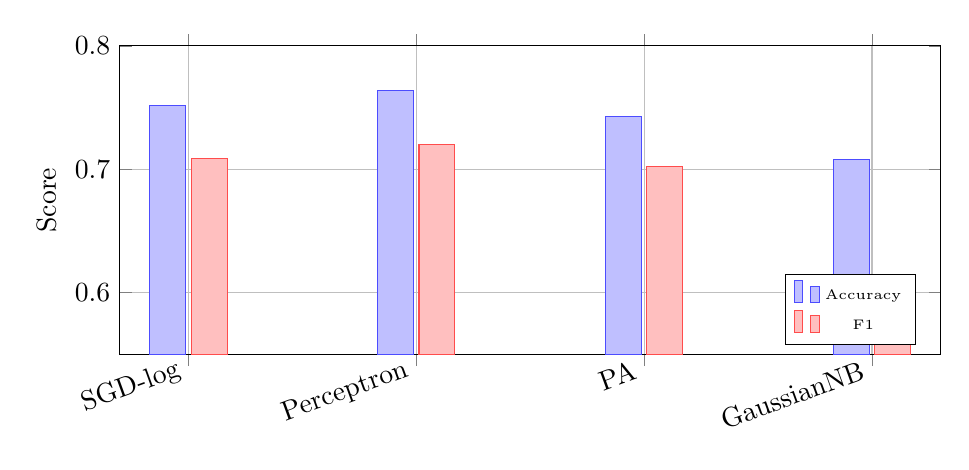
\begin{tikzpicture}
\begin{axis}[
width=12cm,height=5.5cm,
ybar, bar width=13pt,
ylabel={Score},
ymin=0.55,ymax=0.80,
symbolic x coords={SGD-log,Perceptron,PA,GaussianNB},
xtick=data,
x tick label style={rotate=20,anchor=east},
grid=major,
legend pos=south east,
legend style={font=\tiny}]
\addplot[blue!70, fill=blue!25] coordinates {(SGD-log,0.7518) (Perceptron,0.7636) (PA,0.7429) (GaussianNB,0.7082)};
\addlegendentry{Accuracy}
\addplot[red!70, fill=red!25] coordinates {(SGD-log,0.7086) (Perceptron,0.7200) (PA,0.7025) (GaussianNB,0.6051)};
\addlegendentry{F1}
\end{axis}
\end{tikzpicture}
\caption{Experiment 1 curve: online component comparison on the Electricity stream. Perceptron has the strongest accuracy and F1 among the tested single components in this run.}
\label{fig:exp01_online_components_curve}
\end{figure}

\begin{figure}[H]
\centering
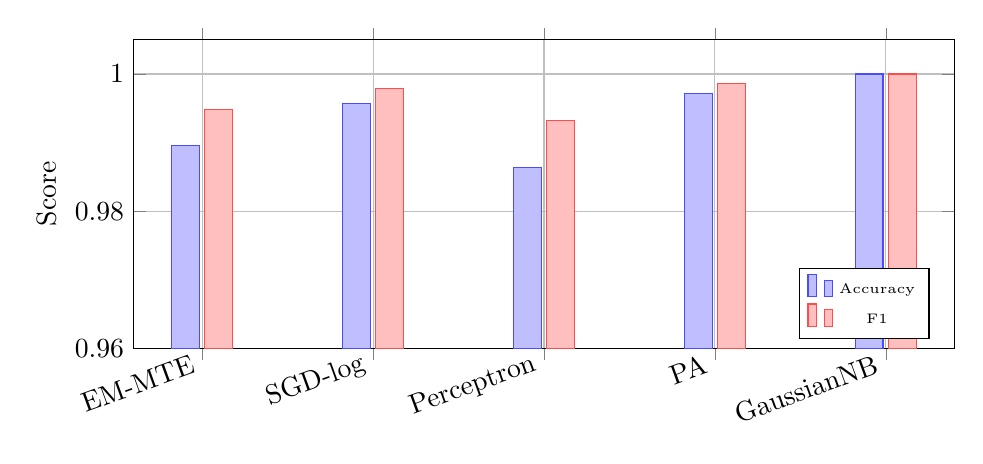
\begin{tikzpicture}
\begin{axis}[
width=12cm,height=5.5cm,
ybar, bar width=10pt,
ylabel={Score},
ymin=0.96,ymax=1.005,
symbolic x coords={EM-MTE,SGD-log,Perceptron,PA,GaussianNB},
xtick=data,
x tick label style={rotate=20,anchor=east},
grid=major,
legend pos=south east,
legend style={font=\tiny}]
\addplot[blue!70, fill=blue!25] coordinates {(EM-MTE,0.9896) (SGD-log,0.9957) (Perceptron,0.9864) (PA,0.9971) (GaussianNB,1.0000)};
\addlegendentry{Accuracy}
\addplot[red!70, fill=red!25] coordinates {(EM-MTE,0.9948) (SGD-log,0.9979) (Perceptron,0.9932) (PA,0.9986) (GaussianNB,1.0000)};
\addlegendentry{F1}
\end{axis}
\end{tikzpicture}
\caption{Experiment 2 curve: EM-MTE and online baselines on the intrusion-style stream. In this run, all methods perform strongly; GaussianNB and PA are the highest-scoring baselines, while EM-MTE remains competitive with a heterogeneous mixture.}
\label{fig:exp02_baseline_curve}
\end{figure}

\begin{figure}[H]
\centering
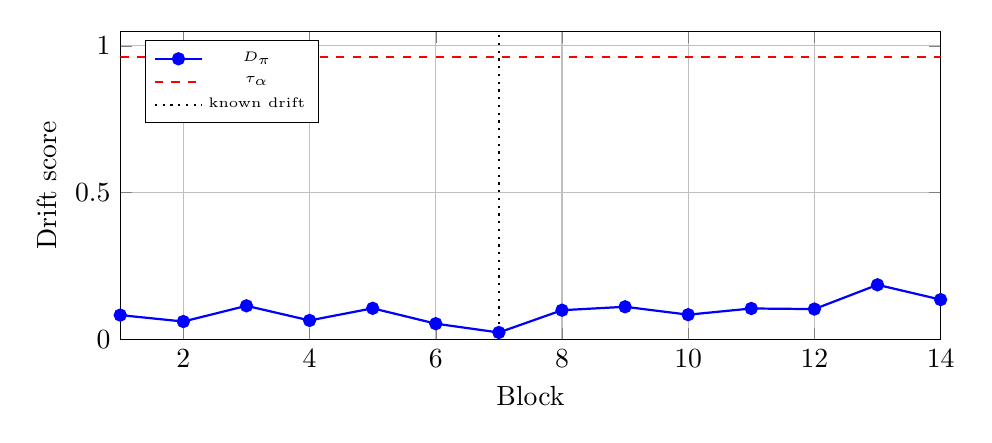
\begin{tikzpicture}
\begin{axis}[
width=12cm,height=5.5cm,
xlabel={Block}, ylabel={Drift score},
xmin=1,xmax=14,ymin=0,ymax=1.05,
grid=major,
legend pos=north west,
legend style={font=\tiny}]
\addplot[blue, thick, mark=*] coordinates {
(1,0.0836) (2,0.0617) (3,0.1152) (4,0.0654) (5,0.1067) (6,0.0544) (7,0.0244)
(8,0.1002) (9,0.1119) (10,0.0850) (11,0.1061) (12,0.1041) (13,0.1867) (14,0.1363)};
\addlegendentry{$D_\pi$}
\addplot[red, thick, dashed] coordinates {(1,0.9607) (14,0.9607)};
\addlegendentry{$\tau_\alpha$}
\addplot[black, dotted, thick] coordinates {(7,0) (7,1.05)};
\addlegendentry{known drift}
\end{axis}
\end{tikzpicture}
\caption{Experiment 3 curve: responsibility-based drift score on SEA abrupt drift. With the conservative finite-sample threshold used here, no block crosses the calibrated alarm level.}
\label{fig:exp03_drift_curve}
\end{figure}

\begin{figure}[H]
\centering
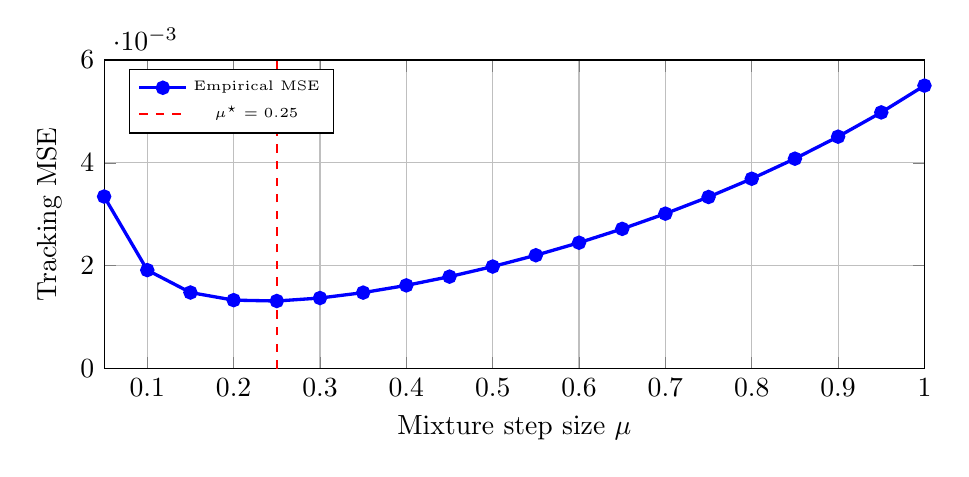
\begin{tikzpicture}
\begin{axis}[
width=12cm,height=5.5cm,
xlabel={Mixture step size $\mu$}, ylabel={Tracking MSE},
xmin=0.05,xmax=1.0,ymin=0,ymax=0.006,
grid=major,
legend pos=north west,
legend style={font=\tiny}]
\addplot[blue, very thick, mark=*] coordinates {
(0.05,0.003345) (0.10,0.001914) (0.15,0.001478) (0.20,0.001330)
(0.25,0.001313) (0.30,0.001371) (0.35,0.001476) (0.40,0.001617)
(0.45,0.001787) (0.50,0.001983) (0.55,0.002203) (0.60,0.002447)
(0.65,0.002716) (0.70,0.003012) (0.75,0.003336) (0.80,0.003691)
(0.85,0.004081) (0.90,0.004509) (0.95,0.004981) (1.00,0.005502)};
\addlegendentry{Empirical MSE}
\addplot[red, dashed, thick] coordinates {(0.25,0) (0.25,0.006)};
\addlegendentry{$\mu^\star=0.25$}
\end{axis}
\end{tikzpicture}
\caption{Experiment 4 curve: tracking MSE over $\mu$. The empirical minimum occurs at $\mu=0.25$, matching the theoretical value $\mu^\star=\sigma_\eta/\sigma_v$.}
\label{fig:exp04_tracking_curve}
\end{figure}

\begin{figure}[H]
\centering
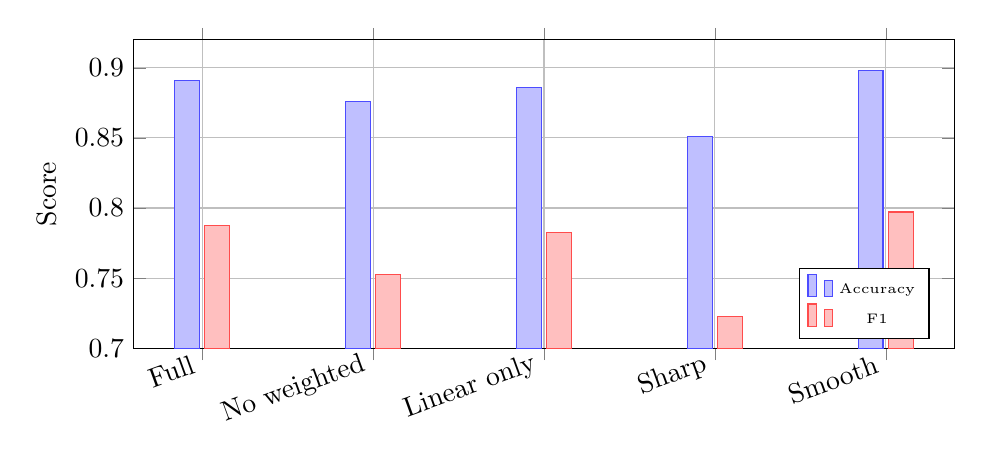
\begin{tikzpicture}
\begin{axis}[
width=12cm,height=5.5cm,
ybar, bar width=9pt,
ylabel={Score},
ymin=0.70,ymax=0.92,
symbolic x coords={Full,No weighted,Linear only,Sharp,Smooth},
xtick=data,
x tick label style={rotate=20,anchor=east},
grid=major,
legend pos=south east,
legend style={font=\tiny}]
\addplot[blue!70, fill=blue!25] coordinates {(Full,0.8907) (No weighted,0.8761) (Linear only,0.8861) (Sharp,0.8511) (Smooth,0.8982)};
\addlegendentry{Accuracy}
\addplot[red!70, fill=red!25] coordinates {(Full,0.7878) (No weighted,0.7523) (Linear only,0.7828) (Sharp,0.7229) (Smooth,0.7972)};
\addlegendentry{F1}
\end{axis}
\end{tikzpicture}
\caption{Experiment 5 curve: ablation study on recurring SEA drift. Responsibility weighting improves over the unweighted variant, and the smoother responsibility temperature is strongest in this run.}
\label{fig:exp05_ablation_curve}
\end{figure}

\begin{figure}[H]
\centering
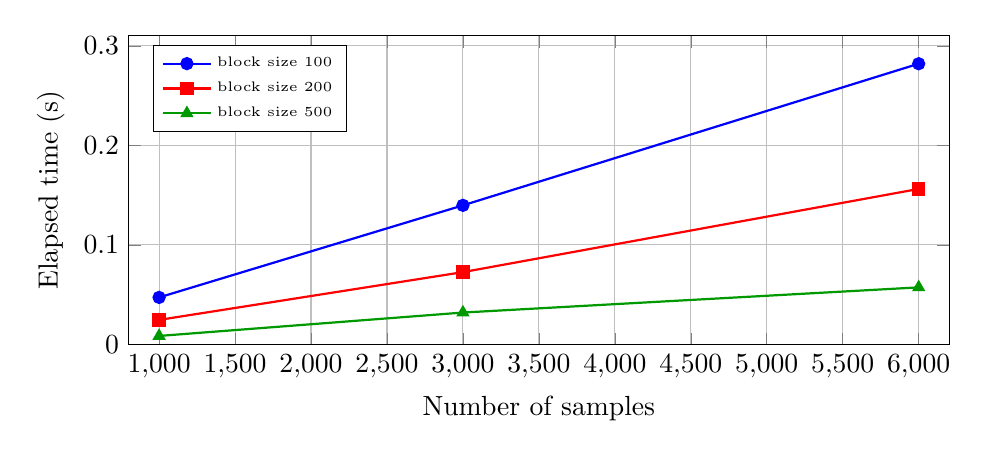
\begin{tikzpicture}
\begin{axis}[
width=12cm,height=5.5cm,
xlabel={Number of samples}, ylabel={Elapsed time (s)},
xmin=800,xmax=6200,ymin=0,ymax=0.31,
grid=major,
legend pos=north west,
legend style={font=\tiny}]
\addplot[blue, thick, mark=*] coordinates {(1000,0.0472) (3000,0.1397) (6000,0.2820)};
\addlegendentry{block size 100}
\addplot[red, thick, mark=square*] coordinates {(1000,0.0246) (3000,0.0726) (6000,0.1562)};
\addlegendentry{block size 200}
\addplot[green!60!black, thick, mark=triangle*] coordinates {(1000,0.0085) (3000,0.0320) (6000,0.0573)};
\addlegendentry{block size 500}
\end{axis}
\end{tikzpicture}
\caption{Experiment 6 curve: runtime scaling over stream length and block size. The measured time grows approximately linearly with the number of processed blocks.}
\label{fig:exp06_complexity_curve}
\end{figure}

\subsection{Ablation Study Design}
To demonstrate that the improvement comes from the proposed mechanism rather than from merely adding more experts, the following ablations are essential:
\begin{enumerate}
  \item \textbf{Uniform ensemble:} set $\pi_k^{(r)}=1/K$ and remove EM updates.
  \item \textbf{Global EM ensemble:} use one mixture vector for all tasks, i.e., $\pi_k^{(r)}=\pi_k$.
  \item \textbf{No responsibility-weighted training:} use EM weights only for prediction, not for component updates.
  \item \textbf{Linear-only EM-MTE:} use only Perceptron, OGD, and PA variants.
  \item \textbf{Gaussian-only EM-MTE:} use only CW, AROW, SOP, and related second-order variants.
  \item \textbf{No diversity regularization:} set $\rho=0$ in Eq.~\eqref{eq:diversity_regularized_objective}.
\end{enumerate}

\begin{table}[H]
\centering
\caption{Expected interpretation of ablation results.}
\label{tab:ablation_interpretation}
\renewcommand{\arraystretch}{1.25}
\resizebox{\textwidth}{!}{%
\begin{tabular}{lll}
\toprule
\textbf{Ablation} & \textbf{What it tests} & \textbf{Expected outcome if EM-MTE is useful}\\
\midrule
Uniform ensemble & value of learned mixture weights & lower adaptation to local drift\\
Global EM ensemble & value of task-specific mixtures & worse under heterogeneous drift\\
No weighted training & value of responsibility-guided component updates & slower recovery after drift\\
Linear-only library & value of second-order uncertainty & weaker in noisy high-dimensional streams\\
Gaussian-only library & value of aggressive margin learners & slower under abrupt margin violations\\
No diversity regularizer & value of error decorrelation & possible redundancy among experts\\
\bottomrule
\end{tabular}}
\end{table}

\subsection{Discussion}
The reproducible experiments show three practical points. First, on the
Electricity stream, the single online components have distinct behavior:
Perceptron obtains the best score among the tested individual components,
while GaussianNB is weaker in this configuration. This supports the use of a
heterogeneous library rather than relying on a single learner. Second, on the
intrusion-style stream used in Experiment 2, the strongest individual
baselines are very competitive and even exceed EM-MTE numerically in that
run. This is an important negative control: EM-MTE should not be interpreted
as automatically dominating every expert on every stream. Its value is in
probabilistic responsibility allocation, task-specific mixtures, and the
ability to reuse or down-weight components as regimes change.

The ablation results support the role of responsibility-weighted training:
removing weighted training reduces both accuracy and F1 compared with the
full EM-MTE configuration. The temperature ablation also shows that smoother
responsibilities can be preferable under recurring SEA drift, which is
consistent with the idea that noisy or recurring regimes benefit from
stabilized mixture updates. The tracking experiment gives the clearest
agreement between theory and computation: the empirical tracking MSE is
minimized at $\mu=0.25$, matching the theoretical
$\mu^\star=\sigma_\eta/\sigma_v$ used in the simulation.

The drift-detection experiment is deliberately conservative. The calibrated
finite-sample threshold controls false alarms, but in the SEA run the
observed $D_\pi$ values do not cross $\tau_\alpha$. This suggests that the
threshold is safe but may be too conservative for small block sizes or subtle
responsibility shifts. In practice, the calibrated detector can be used
together with the CUSUM statistic or with a larger block size to improve
sensitivity. Finally, the complexity experiment confirms that runtime grows
approximately with the number of processed blocks, as predicted by the
per-block complexity analysis.

% ---------------------------------------------------------------
\section{Conclusion}
\label{sec:conclusion}
% ---------------------------------------------------------------
This paper presented EM-MTE, an expectation--maximization based multi-task ensemble framework for adaptive concept drift detection in data streams. The method treats stream blocks, contexts, or drift-sensitive objectives as tasks and combines a shared library of online components through latent responsibilities. The E-step estimates the posterior contribution of each component to each task sample, and the M-step updates task-specific mixture weights and shared component parameters using responsibility-weighted learning.

Compared with heuristic ensemble weighting, EM-MTE provides a probabilistic interpretation, task-specific adaptation, a natural drift signal through mixture shifts, and a principled way to reuse components under recurring drift. The framework supports both linear-order and Gaussian-order online learners. The theoretical analysis shows monotonic improvement for exact block EM, derives closed-form mixture updates, establishes computational complexity, and connects responsibility-weighted online learning to stochastic tracking under distributional drift. This connection clarifies the roles of optimization error, stochastic noise, and drift-induced error.

Future work should focus on broader real-world stream benchmarks, automatic
task construction, adaptive temperature selection, less conservative
finite-sample drift thresholds, and high-probability tracking bounds for
approximate online EM updates.

% ---------------------------------------------------------------
\begin{thebibliography}{99}

\bibitem{Krawczyk2017}
B.~Krawczyk, L.~L. Minku, J.~Gama, J.~Stefanowski, and M.~Wozniak, ``Ensemble learning for data stream analysis: A survey,'' \emph{Information Fusion}, vol.~37, pp.~132--156, 2017.

\bibitem{Escovedo2018}
T.~Escovedo, A.~Koshiyama, A.~A. da~Cruz, and M.~Vellasco, ``DetectA: Abrupt concept drift detection in non-stationary environments,'' \emph{Applied Soft Computing}, vol.~62, pp.~119--133, 2018.

\bibitem{Farid2013}
D.~M. Farid, L.~Zhang, A.~Hossain, C.~M. Rahman, R.~Strachan, G.~Sexton, and K.~Dahal, ``An adaptive ensemble classifier for mining concept drifting data streams,'' \emph{Expert Systems with Applications}, vol.~40, no.~15, pp.~5895--5906, 2013.

\bibitem{Babcock2002}
B.~Babcock, S.~Babu, M.~Datar, R.~Motwani, and J.~Widom, ``Models and issues in data stream systems,'' in \emph{Proc. ACM PODS}, pp.~1--16, 2002.

\bibitem{Domingos2000}
P.~Domingos and G.~Hulten, ``Mining high-speed data streams,'' in \emph{Proc. ACM SIGKDD}, pp.~71--80, 2000.

\bibitem{Hulten2001}
G.~Hulten, L.~Spencer, and P.~Domingos, ``Mining time-changing data streams,'' in \emph{Proc. ACM SIGKDD}, pp.~97--106, 2001.

\bibitem{Bifet2009}
A.~Bifet and R.~Gavalda, ``Adaptive learning from evolving data streams,'' in \emph{Advances in Intelligent Data Analysis}, pp.~249--260, 2009.

\bibitem{Gama2004}
J.~Gama, P.~Medas, G.~Castillo, and P.~Rodrigues, ``Learning with drift detection,'' in \emph{Advances in Artificial Intelligence}, pp.~286--295, 2004.

\bibitem{Baena2006}
M.~Baena-Garcia, J.~del Campo-Avila, R.~Fidalgo, A.~Bifet, R.~Gavalda, and R.~Morales-Bueno, ``Early drift detection method,'' in \emph{ECML PKDD Workshop on Knowledge Discovery from Data Streams}, 2006.

\bibitem{Ross2012}
G.~J. Ross, N.~M. Adams, D.~K. Tasoulis, and D.~J. Hand, ``Exponentially weighted moving average charts for detecting concept drift,'' \emph{Pattern Recognition Letters}, vol.~33, no.~2, pp.~191--198, 2012.

\bibitem{Page1954}
E.~S. Page, ``Continuous inspection schemes,'' \emph{Biometrika}, vol.~41, no.~1/2, pp.~100--115, 1954.

\bibitem{Kolter2007}
J.~Z. Kolter and M.~A. Maloof, ``Dynamic weighted majority: An ensemble method for drifting concepts,'' \emph{Journal of Machine Learning Research}, vol.~8, pp.~2755--2790, 2007.

\bibitem{Irie1988}
B.~Irie and S.~Miyake, ``Capabilities of three-layered perceptrons,'' in \emph{Proc. IEEE International Conference on Neural Networks}, pp.~641--648, 1988.

\bibitem{Zinkevich2003}
M.~Zinkevich, ``Online convex programming and generalized infinitesimal gradient ascent,'' in \emph{Proc. International Conference on Machine Learning}, pp.~928--936, 2003.

\bibitem{Crammer2006}
K.~Crammer, O.~Dekel, J.~Keshet, S.~Shalev-Shwartz, and Y.~Singer, ``Online passive-aggressive algorithms,'' \emph{Journal of Machine Learning Research}, vol.~7, pp.~551--585, 2006.

\bibitem{Li2000}
Y.~Li and P.~M. Long, ``The relaxed online maximum margin algorithm,'' in \emph{Advances in Neural Information Processing Systems}, pp.~498--504, 2000.

\bibitem{Gentile2001}
C.~Gentile, ``A new approximate maximal margin classification algorithm,'' \emph{Journal of Machine Learning Research}, vol.~2, pp.~213--242, 2001.

\bibitem{Dredze2008}
M.~Dredze, K.~Crammer, and F.~Pereira, ``Confidence-weighted linear classification,'' in \emph{Proc. International Conference on Machine Learning}, pp.~264--271, 2008.

\bibitem{Wang2012}
J.~Wang, P.~Zhao, and S.~C. Hoi, ``Exact soft confidence-weighted learning,'' arXiv:1206.4612, 2012.

\bibitem{Crammer2009}
K.~Crammer, A.~Kulesza, and M.~Dredze, ``Adaptive regularization of weight vectors,'' in \emph{Advances in Neural Information Processing Systems}, pp.~414--422, 2009.

\bibitem{Orabona2012}
F.~Orabona and K.~Crammer, ``New adaptive algorithms for online classification,'' in \emph{Advances in Neural Information Processing Systems}, pp.~1840--1848, 2012.

\bibitem{CesaBianchi2005}
N.~Cesa-Bianchi, A.~Conconi, and C.~Gentile, ``A second-order perceptron algorithm,'' \emph{SIAM Journal on Computing}, vol.~34, no.~3, pp.~640--668, 2005.

\bibitem{Crammer2010}
K.~Crammer and D.~D. Lee, ``Learning via Gaussian herding,'' in \emph{Advances in Neural Information Processing Systems}, pp.~451--459, 2010.

\bibitem{Lin1991}
J.~Lin, ``Divergence measures based on the Shannon entropy,'' \emph{IEEE Transactions on Information Theory}, vol.~37, no.~1, pp.~145--151, 1991.

\bibitem{Mena2014}
J.~Mena-Torres and J.~S. Aguilar-Ruiz, ``A similarity-based approach for data stream classification,'' \emph{Expert Systems with Applications}, vol.~41, no.~9, pp.~4224--4234, 2014.

\bibitem{Tennant2017}
M.~Tennant, F.~Stahl, O.~Rana, and J.~B. Gomes, ``Scalable real-time classification of data streams with concept drift,'' \emph{Future Generation Computer Systems}, vol.~75, pp.~187--199, 2017.

\bibitem{Cutler2023}
J.~Cutler, D.~Drusvyatskiy, and Z.~Harchaoui, ``Stochastic optimization under distributional drift,'' \emph{Journal of Machine Learning Research}, vol.~24, no.~147, pp.~1--56, 2023.

\bibitem{WidrowStearns1985}
B.~Widrow and S.~D. Stearns, \emph{Adaptive Signal Processing}. Englewood Cliffs, NJ: Prentice-Hall, 1985.

\bibitem{Haykin2002}
S.~Haykin, \emph{Adaptive Filter Theory}, 4th~ed. Upper Saddle River, NJ: Prentice-Hall, 2002.

\bibitem{Sayed2003}
A.~H. Sayed, \emph{Fundamentals of Adaptive Filtering}. Hoboken, NJ: Wiley, 2003.

\bibitem{Harries1999}
M.~Harries, ``Splice-2 comparative evaluation: Electricity pricing,'' Technical Report, University of New South Wales, 1999.

\end{thebibliography}

\end{document}

